% add option draft to skip images
\documentclass[12pt,a4paper,twosided,openany]{scrbook}
%\documentclass[12pt,a4paper,twosided,open=right]{scrbook}
% \documentclass[12pt,a4paper,twosided,open=right,draft]{scrbook}

% Entwickelt auf Basis von Carsten Kerns Template.

\usepackage[backend=biber,style=alphabetic,maxalphanames=60,maxbibnames=10]{biblatex}
% \usepackage[backend=bibtex,style=alphabetic]{biblatex}
% \usepackage{natbib}
\usepackage[ngerman]{babel}
\usepackage[utf8]{inputenc}
\usepackage{csquotes}
\usepackage{ifthen}
\usepackage{xargs}
\usepackage{amsmath}
\usepackage{amsfonts}
\usepackage{amssymb}
\usepackage{graphicx}
\usepackage{svg}
% \usepackage{fancyhdr}
\usepackage{tabularx}
\usepackage{geometry}
\usepackage{setspace}
\usepackage[right]{eurosym}
\usepackage[printonlyused]{acronym}
\usepackage{subfig}
\usepackage{floatflt}
%\usepackage{color}
\usepackage{xcolor}
\usepackage{colortbl}
\usepackage{paralist}
\usepackage{array}
\usepackage{multirow}
% \usepackage{titlesec}
\usepackage{parskip}
% \usepackage[subfigure,titles]{tocloft}
\usepackage[pdfpagelabels=true,colorlinks=true,linkcolor=black,anchorcolor=black,citecolor=black,filecolor=black,menucolor=black,runcolor=black,urlcolor=black]{hyperref}
\usepackage{booktabs}
\usepackage[lighttt]{lmodern}
\usepackage{mathabx}

\usepackage{listings}
\lstset{basicstyle=\footnotesize, captionpos=b, breaklines=true, showstringspaces=false, tabsize=2, frame=lines, numbers=left, numberstyle=\tiny, xleftmargin=2em, framexleftmargin=2em}

\geometry{a4paper, top=27mm, left=25mm, right=15mm, bottom=27mm, headsep=10mm, footskip=12mm}

% make lstinline be normalsize but keep displayed listings small
\makeatletter
\lstdefinestyle{mystyle}{
  basicstyle=%
    \ttfamily
    \lst@ifdisplaystyle\scriptsize\fi
}
\makeatother

\lstset{
	language=C++,
	% basicstyle=\ttfamily\scriptsize,
	style = mystyle,
	% basicstyle=\ttfamily\scriptsize,
	keywordstyle=\bfseries\ttfamily,
	% commentstyle=\color{LimeGreen}\ttfamily,
	commentstyle=\color{gray}\ttfamily,
	emphstyle={\color{Purple!90!black}},
	tabsize=4,
	morekeywords={nullptr,nullptr_t,vector,string,std,list,map,pair,set,size_t,endl,cout,move},
	emph={},
	showstringspaces=false,
}

\setcapindent{0pt}
\setkomafont{captionlabel}{\bfseries}

\DefineBibliographyStrings{ngerman}{
	andothers = {{et\,al\adddot}},
}


\DeclareLabelalphaTemplate{
  \labelelement{
    \field[final]{shorthand}
    \field{label}
    \field[strwidth=3,strside=left,ifnames=1,names=1]{labelname}
    \field[strwidth=1,strside=left,names=1-3]{labelname}
  }
  \labelelement{
    \field[strwidth=2,strside=right]{year}
  }
}
\renewcommand*\labelalphaothers{$^\Asterisk\mkern-.8mu$}

\newcommandx{\student}[3][]{
	\def\studentName{#1}%
	\def\studentMatnr{#2}%
	\def\studentStudiengang{#3}%
}

\newcommandx{\MyTitelseite}[8][]{
\thispagestyle{empty}
\ifthenelse{\equal{#1}{}}{
	
\includegraphics[scale=0.2]{lib/oth-logo.png}
}{
	
\includegraphics[scale=0.2]{lib/oth-logo.png}\hfill\includegraphics[scale=0.5]{#1}
}
\begin{center}
\ifthenelse{\equal{#2}{2}}{ % then
	\vspace*{2cm}
	\Large
	\textbf{Ostbayerische Technische Hochschule Regensburg}\\
	\textbf{Fakultät für Informatik und Mathematik}\\
	\vspace*{2cm}
	\Huge
	\textbf{#3}\\[1em]
	\large
	Zur Erlangung des akademischen Grades des\\
	\ifthenelse{\equal{#3}{Bachelorarbeit}}{Bachelor of Science (B.Sc.)}{Master of Science (M.Sc.)}\\
	\vspace*{1cm}
	\Large
	\textbf{#4}\\
}{ % else
	\vspace*{1cm}
	\Large
	\textbf{#4}\\
	\vspace*{2cm}
	\large
	An der Fakultät für Informatik und Mathematik der\\
	Ostbayerischen Technischen Hochschule Regensburg\\
	im Studiengang\\[2em]
	\textbf{\studentStudiengang}\\[2em]
	eingereichte\\
	\vspace*{1cm}
	\Large
	\textbf{#3}\\[2em]
	\large
	zur Erlangung des akademischen Grades des\\
	\ifthenelse{\equal{#3}{Bachelorarbeit}}{Bachelor of Science (B.Sc.)}{Master of Science (M.Sc.)}
	\vspace*{1cm}
	\Large
}
	\vfill
	\normalsize
	%\newcolumntype{x}[1]{>{\raggedleft\arraybackslash\hspace{0pt}}p{#1}}
	\begin{tabular}{rl}%{6cm}p{7.5cm}}
	    \rule{0mm}{1ex}\textbf{Vorgelegt von:} & \studentName \\
		\rule{0mm}{1ex}\textbf{Matrikelnummer:} & \hspace*{-0.5em}\begin{tabular}[t]{r}\studentMatnr\end{tabular} \\ 
		\ifthenelse{\equal{#2}{1}}{~\\}{\rule{0mm}{1ex}\textbf{Studiengang:} & \studentStudiengang \\[2em]}
		\rule{0mm}{1ex}\textbf{Erstgutachter:} & #5 \\ 
		\rule{0mm}{1ex}\textbf{Zweitgutachter:} & #6 \\[2em]
		\rule{0mm}{1ex}\textbf{Abgabedatum:} & #7 \\ 
	\end{tabular} 
\end{center}
\pagebreak
}



% ein paar nützliche Kommandos

\newcommand\defsec[1]{\label{sec:#1}}
\newcommand\refsec[1]{\ref{sec:#1}}

%\newcommand\todo[1]{\textcolor{red}{[{\textbf{TODO}} #1]}}
\newcommand\todo[1]{} % remove todos

%\newcommand\new[1]{\textcolor{new}{{#1}}}
\newcommand\new[1]{#1} % plain text
%\newcommand\old[1]{\textcolor{gray}{{\sout{#1}}}}
\newcommand\old[1]{} % remove old stuff

\definecolor{lgdv}{rgb}{.80,.23,.13}
\definecolor{agreen}{rgb}{.2,.8,.2}
\definecolor{jorange}{rgb}{.9,.6,.0}
\definecolor{new}{rgb}{.8,.4,.4}

\newcommand\NOTE[3]{\textcolor{#1}{[#2: #3]}}
\newcommand{\TODO}[1]{\\ \colorbox{yellow}{TODO: #1}\\}

%\newcommand\kai[1]{\NOTE{lgdv}{Kai}{#1}}
\newcommand\kai[1]{} % remove notes
%\newcommand\niko[1]{\NOTE{jorange}{Niko}{#1}}
\newcommand\niko[1]{} % remove notes

\newcommand\To{\ensuremath{\to}}
\newcommand\hi[1]{\textcolor{red}{#1}}

\let\shortcite=\cite

\addbibresource{bib.bib}

\begin{document}

% ----------------------------------------------------------------------------------------------------------
% Titelseite
% ----------------------------------------------------------------------------------------------------------
\newcommand{\stud}{Emanuel Erben}  % Ihr Name
\student{\stud}
{3174817}						% Matrikelnummer
{Informatik}					% Studiengang

\MyTitelseite{}					% Optionales Logo des extern betreuenden Unternehmens
% \MyTitelseite{pics/mathcomm}	% Optionales Logo des extern betreuenden Unternehmens
{1}								% Style der Titelseite (1 oder 2)
{Bachelorarbeit}				% Typ der Abschlussarbeit (\in {Bachelorarbeit, Masterarbeit})
{Vergleich verschiedener Ansätze der Multiplattform Applikationsentwicklung anhand einer Beispiel-Anwendung}				% Thema der Arbeit						
{Prof.\ Dr.-Ing.\ Kai Selgrad}		% Betreuer
{Prof.\ Dr.\ Name des Zweitgutachters}	% Zweitgutachter
{15.09.\the\year}				% Abgabedatum

\thispagestyle{empty}
~\pagebreak

\setcounter{page}{1} 

Das muss an den Kapiteln noch gemacht werden:

0.Abstract:
Ende nochmal umschreiben
1.Motivation:
Einordnung nochmal anschauen und insgesamt überarbeiten.
Die Arbeitsbeschreibung

Related:
Überarbeiten und eventuell Performance Untersuchung mit neuem Austauschen.

3.Grundlagen:
Projektbeschreibung : 
noch machen
Themenabgrenzung :
Mal schauen ob noch mehr und bei Spiel Ende nochmal nachschauen.
Erklärung warum nur Smartphone Applikationen betrachtet.
Begriffe:
umstellen
Arten:
Nativ und Hybrid soweit an Selgrad, Rest muss überareiten
drüberlesen

4. Einleitung
Vielleicht nochmal bisl spannender
4.1 Nativ

4.2 hybrid

4.3 Flutter
ausmisten
ordentlich neu schreiben

4.4 hybrid flutter

5.Auswertung
Noch komplett
kriterien aussuchen
Werte zusammenschreiben, messen oder nachforschen
Tabellen und sonstiges erstellen

6.Fazit
Noch komplett


% ----------------------------------------------------------------------------------------------------------
% Abstract
% ----------------------------------------------------------------------------------------------------------
% \thispagestyle{empty}
\setstretch{1.15} % Zeilenspacing
\chapter*{Abstract}

\bigskip 

In den letzten Jahren nutzen viele Leute nicht mehr ihren Computer sondern vor allem ihre Smartphones und andere mobile Endgeräte, um auf verschiedenen Dienste, Konten und Online-Anwendungen zuzugreifen. Um eine Anwendung auf verschiedenen Plattformen veröffentlichen zu können haben Entwickler unterschiedliche Möglichkeiten. Diese reichen dabei von der Entwicklung einer eigenen Anwendung für jede einzelne Plattform bis hin zu einem Code der für die verschiedenen Plattformen genutzt werden kann. Dadurch ist die Wahl des richtigen Entwicklungsansatzes und der Technologie schwer, da jeder Ansatz seine Vor- und Nachteile hat. 

In dieser Arbeit werden vier verschiedene Applikationen, die mit unterschiedlichen Ansätzen implementiert wurden, beschrieben und analysiert. Danach werden die Ergebnisse der verschiedenen Untersuchungen vorgestellt und verglichen. Dabei wird darauf eingegangen, welche Vor- und Nachteile die einzelnen Implementierungen für die betrachteten Kriterien haben. Der Schwerpunkt der Arbeit liegt dabei auf der Android Plattform und speziell den Programmiersprachen Kotlin und Dart. Die vier Implementierungen sind eine native, hybride, cross-kompilierte und eine cross-kompilierte Applikation mit Webanteil, also einem Mix aus hybridem und cross-kompilierten Ansatz.

\frontmatter

% ----------------------------------------------------------------------------------------------------------
% Inhaltsverzeichnis
% ----------------------------------------------------------------------------------------------------------
\tableofcontents
\vfill
\pagebreak

% % ----------------------------------------------------------------------------------------------------------
% % Abbildungsverzeichnis
% % ----------------------------------------------------------------------------------------------------------
\listoffigures
\vfill
\pagebreak
% 
% % ----------------------------------------------------------------------------------------------------------
% % Tabellenverzeichnis (optional)
% % ----------------------------------------------------------------------------------------------------------
% \listoftables
% \vfill
% \pagebreak

% ----------------------------------------------------------------------------------------------------------
% Listingsverzeichnis (optional; Code nur, wenn wirklich sinnvoll und wichtig)
% ----------------------------------------------------------------------------------------------------------
%\lstlistoflistings
%\vfill
%\pagebreak


% ----------------------------------------------------------------------------------------------------------
% Inhalt
% ----------------------------------------------------------------------------------------------------------
\setstretch{1.15}


\mainmatter

\chapter{Motivation}
Wenn eine Applikation entwickelt werden soll, ist die Wahl der richtigen Methode, Frameworks oder auch der Programmiersprache eine wichtige Entscheidung für das Projekt. Viele Entscheidungen können im Verlauf der Entwicklung noch einfach geändert werden, aber um eine derartige Entscheidung zu ändern, müssen Teile der Anwendung oder auch der komplette Quellcode neu geschrieben werden. Dazu kommen tausende Artikel, warum die eine neue Programmiersprache der neue Standard ist. So ist eine derartig wichtige Entscheidung oft sehr schwierig.

Da oft Anwendungen nicht nur auf einem Gerätetyp laufen sollen, sondern allen Nutzern auf den verschiedensten Plattformen zur Verfügung stehen soll, hat diese Entscheidung noch einmal eine größere Bedeutung, da sie auch eng verbunden mit den Kosten der Entwicklung und der Erfahrung durch den Nutzer ist.

In Zeiten der Heimcomputer und des stetig wachsenden Internets war der einfachste Weg , eine Webseite zu entwickeln, die über den Browser der genutzten Geräte aufgerufen werden konnte. Mit der Ära der Smartphones jedoch änderte sich das. So waren Webapplikationen oft nicht für die Nutzung an derartig kleinen Geräten mit einer Toucheingabe angepasst.

Die Nutzung von Smartphones öffnete außerdem die Tür, andere Funktionalitäten wie die Kamera, Bluetooth oder GPS-Daten zu nutzen. Deshalb wurden Applikationen oft mit Objectiv-C beziehungsweise Swift für iOS und Java, jedoch mittlerweile Kotlin für Android entwickelt. Mit deren Hilfe wurden native Anwendungen für das Smartphone entwickelt, die diese neuen mobilen Plattformen optimal ausnutzen konnten.

Durch den Wunsch nach einer Multi-Plattform Anwendung, also dass die App für mehrere Plattformen veröffentlicht werden soll, muss jedoch für jede Plattform eine eigene Applikationen in der jeweiligen Programmiersprache und Technologie geschrieben werden. Dadurch entsteht ein sehr hoher Aufwand und die Kosten multiplizieren sich mit der Zahl der abzudeckenden Plattform. Deswegen wurde bereits früh mit der Entwicklung von sogenannten Cross-Plattform Technologien gestartet, die es ermöglichen sollen, mit einem geteilten Code so viele Plattformen wie möglich abzudecken. So erschien 2008 etwa PhoneGap. Es war ein Open-Source Framework zur Entwicklung von hybriden mobilen Applikationen, die mit Hilfe von HTML, CSS und Javascript programmiert wurden. PhoneGap und sein Nachfolger Cordova waren einige Zeit auch sehr beliebt in diesem Bereich. 2019 hatten beide zusammen einen Marktanteil von knapp 40\% unter den Cross-Plattform Frameworks \cite{statist_CP_Framework}.

Dennoch werden viele Entwicklung immer noch nativ entwickelt. So ergab eine interne Untersuchung der Firma \verb|ScanBot SDK|\footnote{https://scanbot.io/de/blog/native-apps-vs-cross-platform/}, dass 2019 57\% ihrer Nutzer native Applikationen entwickelten, obwohl ihr Produkt ebenso für viele der gängigen Cross-Plattform Frameworks zur Verfügung steht. Außerdem kann in Blogposts von einigen größeren Unternehmen lesen, in dem sie erklären, wie sie versuchten eine  Cross-Plattform-Entwicklungen einzuführen, jedoch aus verschiedenen Gründen  wieder einstellten. So etwa auch Airbnb \cite{Airbnb_react_goals}. Sie nutzten das von Facebook mitentwickelte Framework React Native. 2019 hatte dieses Framework einen Marktanteil von 42\%. 
\break
Ihre Ziele waren einfach:
\begin{enumerate}
    \item Schnelleres entwickeln.
    \item Die gleiche Codequalität beibehalten.
    \item Nur noch eine Codebasis.
    \item Die Entwicklererfahrung verbessern.
\end{enumerate}
Jedoch traten während der Entwicklung einige technische Probleme auf, die dazu führten, dass sie ihre Ziele nicht einhalten konnten und 2018 wieder zu einem nativen Ansatz zurückkehrten.

Durch Beispiele wie dieses, waren und sind App-Entwickler oft skeptisch gegenüber derartigen Lösungen, da dies auch immer mit großen Änderungen und hohen Investitionen verbunden sind. Dennoch ist der Wille da und auch die Zahl der Cross-Plattform Entwicklungen nimmt in den letzten Jahren zu. So ergab die Untersuchung von \verb|ScanBot SDK|, dass 2021 58\% Cross-Plattform Lösungen nutzten. Auch eine Untersuchung von Jetbrains ergab, dass 2021 53\% aller App Entwickler derartige Technologien nutzen \cite{JetBrains_miscellaneous_2021}.

\begin{figure}[ht]
  \centering
  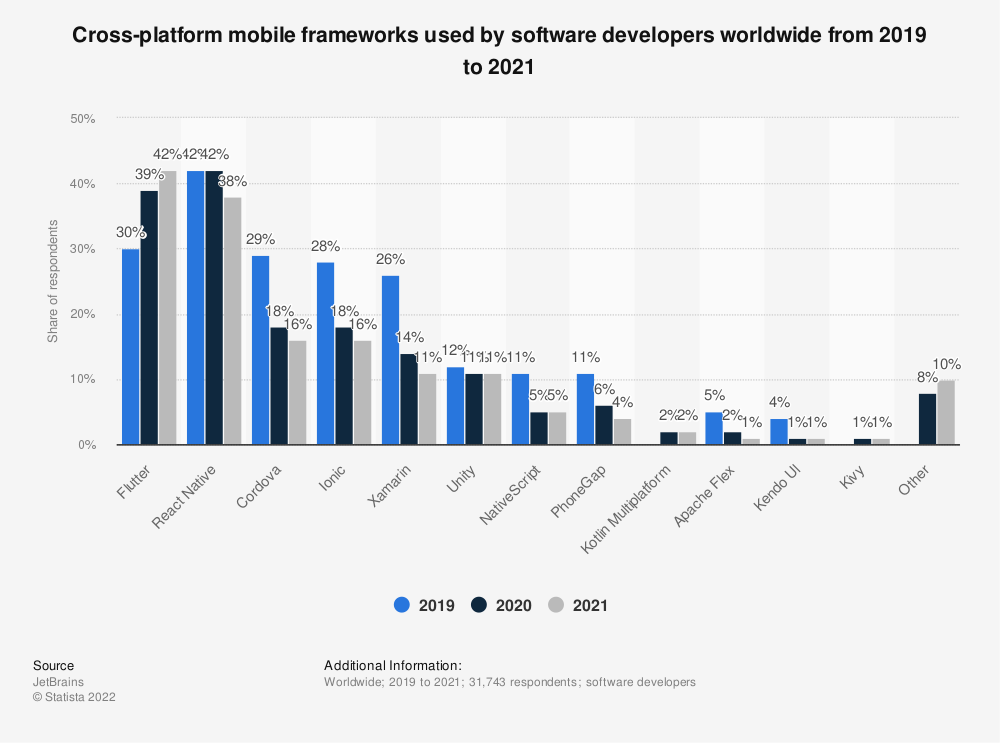
\includegraphics[height=7cm,keepaspectratio]{images/cross-platform-mobile-frameworks.png} 
  \caption[Statistik Cross-Plattform-Frameworks]{Cross-Plattform-Frameworks 2019-2021 \cite{statist_CP_Framework}}
  \label{fig:statista_cross_plattform}
\end{figure}

Diese Zahl könnte sich auch noch stark ändern. Abbildung \ref{fig:statista_cross_plattform} zeigt eine Statistik, die die Verteilung von verschiedenen Cross-Plattform-Entwicklungen zeigt. Sie zeigt eindrucksvoll wie schnell sich die Verteilung von Cross-Platform Frameworks ändern kann. Ein Framework, das hier jedoch besonders auffällt ist Flutter. Es ist ein Framework das erst 2017 auf den Markt gekommen ist und innerhalb von gerade einmal 4 Jahren auf einen Marktanteil von 42\% gekommen ist. Von einigen wird es als der neue Standard angesehen und viele Unternehmen steigen auf Flutter um oder bekunden großes Interesse daran. 

Jedoch gibt es auch Entwickler, die wegen Unsicherheiten und einigen anderen Gründen immer noch nativ entwickeln. So entwickelt die Number42 alle ihrer betreuten mobilen Applikationen mit den nativen Programmiersprachen. Auch die nativen Programmiersprachen entwickeln sich dabei stetig weiter und bekommen Änderungen, die eine Entwicklung vereinfachen und beschleunigen. Dadurch ist auch dieser Ansatz nicht von der Hand zu weisen und es kann durchaus sinnvoll sein, neue Apps weiterhin nativ zu entwickeln.

\section{Einordnung der Arbeit}
Diese Arbeit soll zunächst einen geordneten Überblick über die verschiedenen Entwicklungsansätze geben und somit eine gemeinsame Grundlage bilden, da es viele verschiedene Einordnungen gibt.
Danach soll anhand von verschiedenen Implementierungen eine Untersuchung von vier verschiedenen Ansätzen gemacht werden, um einige der vorgestellten Ansätze genauer zu betrachten.
Am Schluss soll anhand der verschiedenen Implementierungen und Erfahrungen während der Entwicklung ein Vergleich zwischen den ausgewählten Ansätzen gezogen werden und daraus ein Fragekatalog erstellt werden, der die Wahl eines passenden Ansatzes erleichtern soll.


\section{Aufbau der Arbeit}
Diese Arbeit hat 6 Kapitel. Eine Einleitung und Motivation ist in Kapitel 1 zu finden. In Kapitel 2 werden verwandten Arbeiten vorgestellt, während in Kapitel 3 die verschiedenen App-Arten, das Projekt, die verschiedenen Implementierungen vorgestellt und eine Abgrenzung der Arbeit stattfindet.
Danach wird in Kapitel 4 die verschiedenen Implementierungen vorgestellt und einige Bemerkung zu der Entwicklung getroffen, dabei soll auch auf Stärken und Schwächen der einzelnen Implementierungen eingegangen werden, die bei der Implementierung aufgefallen sind.
In Kapitel 5 soll anschließend eine Auswertung der einzelnen Entwicklungsansätze stattfinden und anhand einiger Kriterien und weiterer Erklärungen Ein Vergleich gezogen werden. Zusätzlich wird anhand eines Fragenkatalogs mit Erklärungen ein Entscheidungskompass gegeben, der bei der Auswahl eines Ansatzes helfen soll.  Abschließend soll in Kapitel 6 ein Fazit gezogen werden und ein Ausblick auf künftige Arbeiten aufgezeigt werden.
\chapter{Related Work}
Es gibt einige verschiedene Arbeiten die sich um das Thema Cross-Plattform bzw. Multi-Plattform Entwicklung drehen. Die vorgestellten Arbeiten sind oft Veröffenltichungen im Rahmen von Konferenzen oder andere Wissenschaftliche Arbeiten. Im folgenden sollen einige vorgestellt werden und darauf eingegangen werden, was die Arbeiten von dieser unterscheidet und weshalb diese Arbeit wichtig ist.

\subsubsection{A study on approaches to build cross-platform mobile applications and criteria to select appropriate approach - C.P Rahul Raj \& Seshu Babu Tolety}
In ihrer Arbeit stellen Raj und Tolety zunächst die verschiedenen Arten von Cross-Plattform Entwicklungsansätzen vor. Nachdem sie hier einige vor und Nachteile erläutern gehen sie danach über, zu erläutern wie man eine passende Methode auswählt. Dafür unterscheiden sie zunächst nach der Art der Applikation und unterteilen sie in vier Klassen. Serverdaten-, Sensor bzw. Ein-und Ausgabe gestützte, alleinstehende und Client-Server-Applikationen. Im folgenden erklären sie die verschiedenen Klassen und erläutern jeweils, welchen Ansatz sie am ehesten wählen würden und geben hierfür einige Empfehlungen. So empfehlen sie etwa, dass bei Server gestützten Applikationen grundsätzlich einen Web-gestützten Ansatz empfehlen, da dadurch sowohl das User Interface als auch die Geschäfftslogik komplett genutzt werden kann, ohne sie auf den einzelenen Plattformen neu zu schreiben. Sie schränken dabei jedoch ein, dass sobald die Anwendung selber einen Teil an Funktionalität anbieten soll, ein Hybrider Ansatz der best gewählte wäre. Aus diesen Erklärungen und anderen bildeten sie daraufhin die Entscheidungstabelle, die in Abbildung \ref{fig:decision_table_IEEE_related_work} zu sehen ist. Dabei steht der Wert 1 für nicht empfohlen, 2 empfohlen, aber nicht optimale Methode und 3 perfekte Methode.\cite{IEEE_Rahul_Seshu}

Als Fazit erklären sie dann, dass Cross-Plattform Lösungen die bevorzugte Methodik sind, wenn mehrere Plattformen genutzt werden sollen, wenn Entwicklungszeit und Kosten ein kritischer Faktor sind. Sie sagen asußerdem, dass jeder Ansatz seine eigenen Vor und Nachteile hat und somit eine Entscheidung je nach Applikationsart zu treffen ist. \cite{IEEE_Rahul_Seshu}
\begin{figure}[ht]
  \centering
  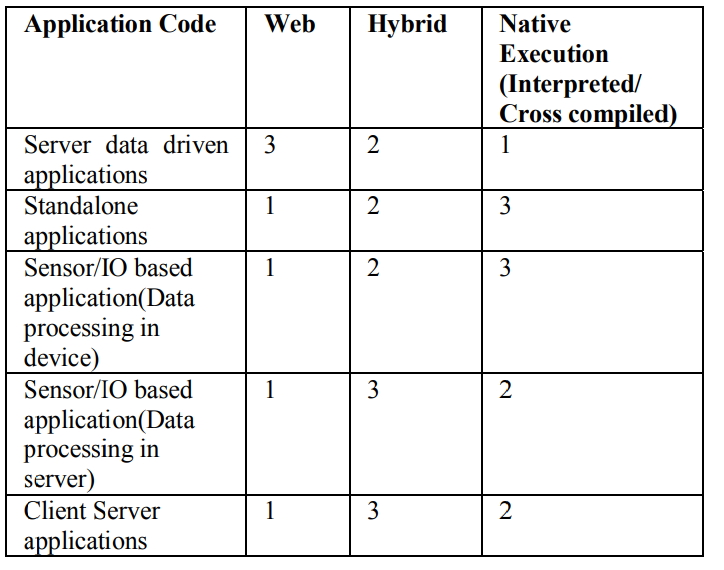
\includegraphics[height=7cm,keepaspectratio]{images/IEEE_related_chapter.jpg} 
  \caption{Entscheidungstabelle für Applikationstyp und bevorzugter Ansatz \cite{IEEE_Rahul_Seshu}}
  \label{fig:decision_table_IEEE_related_work}
\end{figure}

Diese Arbeit stellt einen guten Überblick über einen möglichen Entscheidungsweg dar und erklärt einige wichtige Grundlagen, die zur Unterscheidung bei der Entwicklung von Multi-Plattform-Anwendungen wichtig sind. Jedoch wird einerseits in dieser Arbeit der Aspekt der rein nativen Entwicklung mit den Plattform spezifischen Entwicklungsmethodiken komplett vernachlässigt und die Arbeit stützt sich lediglich auf Recherchen, es wurden jedoch keinerlei Versuche oder messabaren Werte genutzt. Anders ist hier die nächste Arbeit.


\subsubsection{Approaches to mobile application development: Comparative performance analysis - Delia et Al}
Delia et Al vergleichen in ihrer Arbeit die Performance von verschiedenen Ansätzen zur Entwicklung von mobilen Applikationen. Auch sie unterscheiden zunächst, die verschiedenen Klassen der Entwicklungsmethoden. Danach stellen sie ihre Testmethodik vor. Um die Performance der Unterschiedlichen Plattformen zu testen nutzen sie hierfür eine Mathematische Berechnung indem die Summe über 500.000 Schleifendurchläufe einer Berechnung bestehend aus einem Logarithmus, einer Wurzel und Fakultät berechnet wird. Um das ganze etwas differenzierter zu betrachten nutzten sie dafür verschiedene Android und iOS Geräte um die sieben verschiedenen Anwendungen laufen zu lassen. Um die Zeit zu messen, die die Berechnung dauerte, namen sie vor und nach der Ausführung der Berechnung die Zeit und bildeten daraus die Differenz um zu sehen wie lang die jeweiligen Berechnung dauerte. Dies führten sie dann jeweils 30 mal aus und berechneten daraus die Durchschnittliche Laufzeit T und die Standardabweichung S. Das Ergebnis ist in Abbildung \ref{fig:result_table_IEEE_related_work} zu sehen.\cite{IEEE_development_classes}

\begin{figure}[ht]
  \centering
  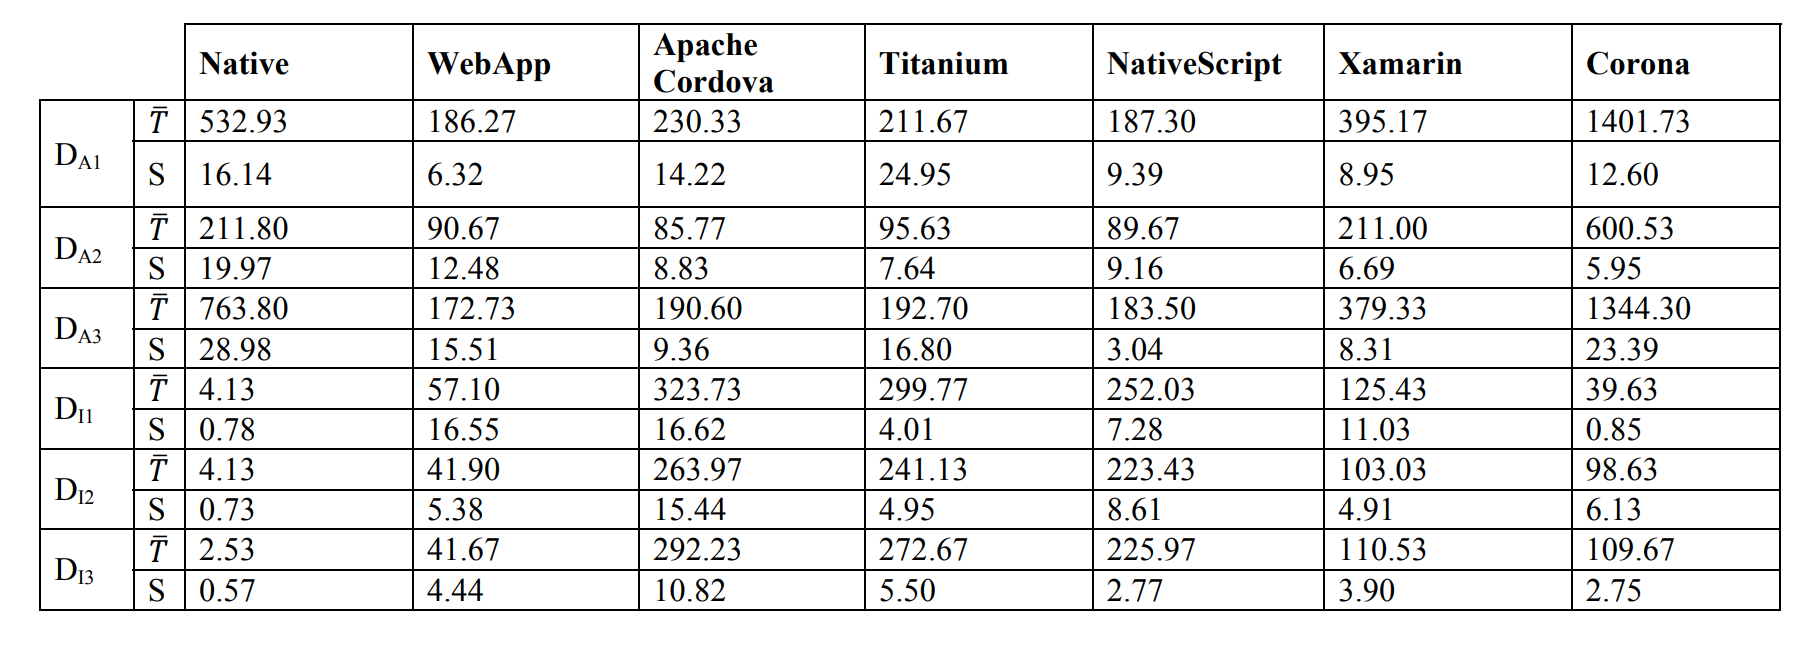
\includegraphics[width=\textwidth,keepaspectratio]{images/IEEE_Delia_Al.png}
  \caption{Ergebnisstabelle der Performancemessungen \cite{IEEE_development_classes}}
  \label{fig:result_table_IEEE_related_work}
\end{figure}

Interessant ist hier vor allem zu sehen, dass es erhebliche Unterschiede zwischen Android und iOS gibt. So ist nicht sichergestellt, dass nur weil ein Ansatz auf Android sehr schnell lief, er auch auf iOS so gut lief. Jedoch erklären sie hierzu selber in der Auswertung ihrer Arbeit, dass ein Vergleich durch die Verwendung verschiedener Hardware schwierig ist.\cite{IEEE_development_classes} Dennoch sagen sie selber, dass die benutzte Implementierung auf iOS effizienter scheint, als die auf Android, was sie auf die Android Runtime zurückführen. Generell stellten sie fest, dass Web-Applikationen in ihren Test die beste Performance über die Geräte hinweg zeigten.\cite{IEEE_development_classes}

In dieser Arbeit wurde lediglich auf die Performance der Applikationen eingegangen. Zu der Webentwicklung gehören jedoch so viel mehr Aspekte, die einen Einfluss auf die Auswahl der Entwicklungsmethode haben. Dazu kommt, dass die Arbeit, da sie 2017 bereits geschrieben wurde, heute komplett anders aussehen könnte/würde. Nicht nur, dass mittlerweile auf beiden Plattformen neue und performantere Programmiersprachen genutzt werden, sondern auch die Geräte von heute haben deutlich schnellere Prozessoren, mehr Arbeitspeicher und vieles mehr. Ein Smartphone von 2017 ist mit einem heutigen nicht mehr vergleichbar. Deswegen rückt der Faktor der Performance immer weiter in den Hintergrun, was auch eine recht neue Untersuchung von 2020 von Bi{\o}rn-Hansen et Al bestätigt. Sie fanden zwar einige Unterschiede zwischen den verschiedenen Frameworks gefunden, kamen aber am Ende zu dem Fazit, dass zwar in der Summe die nativen etwas besser Abschnitten, aber einige hybriden Ansätze in ein paar Aufgaben sogar besser performten als die nativen und kein Ansatz in allen Punkten besser war als die anderen.\cite{BirnHansen.2020}

\subsubsection{Framework Choice Criteria for Mobile Application Development - Khachouch et Al}
Ebenfalls eine neuere Untersuchung ist die folgende von Jhachouch et Al. Ihr Ziel war es dabei einen Entscheidungsgraphen zu erstellen, bei dem man durch Beantwortung einiger Fragen am Ende zu einer Antwort gelangen soll. Sie kritisierten, dass es durchaus einige solcher Graphen gäbe, jedoch dies oft in Richtung eines beworbenen Frameworks manipuliert wären. Deswegen entwickelten sie einen Fragekatalog und Graphen, der keine Aussage zu einem bestimmten Framework oder Technologie einer Firma trifft, sondern dass zu einer Entwicklungsmethodik rät. Das Ergebnis daraus kann man in Abbildung \ref{fig:decision_graph_IEEE_related_work} sehen.\cite{IEEE_Khackouch_Al}

\begin{figure}[ht]
  \centering
  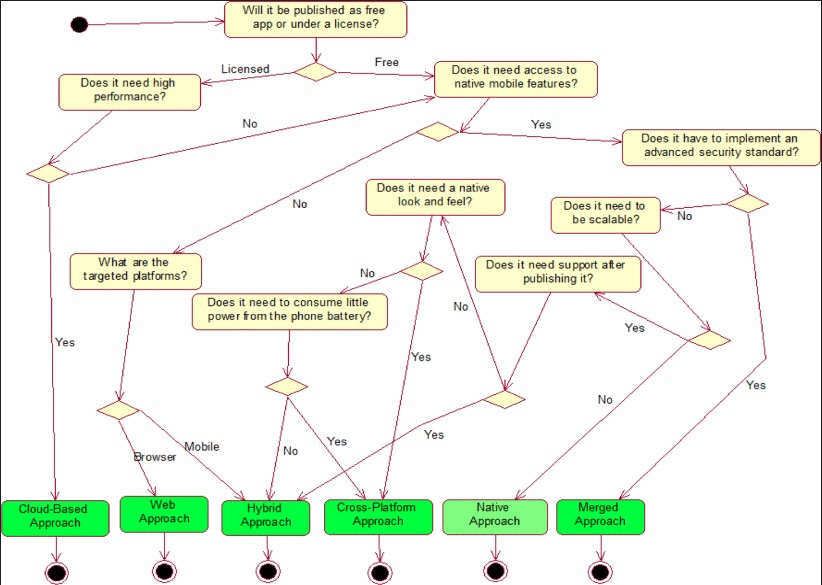
\includegraphics[width=\textwidth,keepaspectratio]{images/IEEE_Khachouch_Decision_Graph.jpg}
  \caption{Entwickelter Entscheidungsgraph von Khachouch et Al \cite{IEEE_Khackouch_Al}}
  \label{fig:decision_graph_IEEE_related_work}
\end{figure}

Sie ziehen am Ende das Fazit, dass wenn "keine Einschränkungen im Bezug auf Kosten oder Personal existieren, der native Ansatz aufgrund seiner Vorteile in Bezug auf Qualität, Leistung und Ergonomie die beste Lösung"\cite{IEEE_Khackouch_Al}{Chapter~4} sei.

Das Problem an dieser Arbeit ist, dass einerseits es in der Realität es nie den Fall geben wird, dass es keine Einschränkungen bei Kosten oder Personal geben wird. Desweiteren ist es auch dann nicht verständlich, warum etwa ein Cross-Plattform Ansatz nicht auch gut sein könnte. Auch die gestellten Fragen und ihre Anworten sind manchmal etwas irritierend. So ist die Frage ob die Anwendung nach einer Veröffentlichung weiterhin Support benötigt. Bei der Antwort Ja wied der Hybride Ansatz empfohlen bei Nein geht es weiter und nach ein bis zwei Fragen wird dann zwischen Hybriden und Cross-Plattform Ansatz entschieden. Jedoch sollte eine App immer weiter unterstützt beziehungsweise gewartet werden. So sollten etwa Sicherheitsupdates von genutzten Bibliotheken oder sonstiges in Apps eingebaut werden können. Auch die Begründung, warum Cross-Plattform Ansätze ein Support nach der Veröffentlichung hier problematisch ist, erklären sie nicht. Sie sagen sogar in ihrer Erläuterung der Fragen, dass alle von ihnen Untersuchten Ansätze einen guten Support anbieten.\cite{IEEE_Khackouch_Al} Ein Argument der hier angebracht werden könnte, ist, dass Cross-Plattformen stark von ihrer Popularität abhängig sind. So können Frameworks eingestellt werden, wenn sie keine aktive Community mehr haben. Jedoch werden selbst dann oft noch durch Open-Source Unterstützer wichtige Updates veröffentlicht um einen Langzeitsupport zu ermöglichen.\TODO{Nochmal überarbeiten. Noch nicht zufrieden.}
\chapter{Grundlagen}
Im folgenden Kapitel werden zunächst einige Begriffe geklärt, die Ausgangssituation dargestellt und das Thema abgesteckt.

\section{Begriffe}
\subsubsection{App/Applikation/Anwendung}
Im Rahmen dieser Arbeit wird oft von einer App oder Applikation geredet. Damit ist eine Anwendung gemeint, die für mobile Endgeräte entwickelt wurden. Die am häufigsten genutzten mobilen Geräte sind dabei Smartphones mit einem Marktanteil von etwa 62,6\%\footnote{https://gs.statcounter.com/os-market-share}.

\subsubsection{Plattform}
Der Begriff Plattform kann auf unterschiedliche Betriebssysteme, Prozessortypen, Kommunikationsprotokolle oder Hardwaresysteme bezogen werden \cite{2014Mulit_plattform_definition}. In dieser Arbeit werden damit die unterschiedlichen Betriebssysteme bezeichnet. Beispiele für diese sind Android, iOS oder auch MacOS.

\subsubsection{Multi-Plattform-Anwendung}
Als Multi-Plattform-Anwendung werden jene Anwendung bezeichnet, die auf mehreren Plattformen ausgeführt werden kann und dabei eine gleiche oder ähnliche Funktionalität hat \cite{2014Mulit_plattform_definition}. Eine Anwendung muss dabei nicht für alle Plattformen implementiert sein. Ist eine Anwendung auf mehr als einer Plattform verfügbar so kann diese als Multi-Plattform-Anwendung bezeichnet werden.

\subsubsection{Cross-Plattform-Anwendung}
Cross-Plattform-Anwendungen sind ebenfalls, wie Multi-Plattform Anwendungen, auf mehr als einer Plattform ausführbar. Der Unterschied besteht darin, dass Cross-Plattform-Anwendungen eine gemeinsame Codebasis besitzen, die es ermöglicht, die Applikation nur einmalig implementieren zu müssen, jedoch mehrere Plattformen damit abdecken zu können \cite{2014_Cross_plattform}.

\subsubsection{GraphQL}
GraphQL\footnote{https://graphql.org/} ist eine von Facebook vorgestellte Schnittstellen-Technologie für Web-Server. Im Gegensatz zur oft genutzten REST-API kann der Client dabei die Struktur und den Aufbau der Antwort festlegen, wodurch das Senden von unnötigen Daten verhindert wird. Die Kommunikation findet dabei mit Hilfe von JSON statt. Eine Untersuchung von Brito et al \cite{IEEE_GraphQL} ergab, dass durch die Verwendung von GraphQL eine Reduktion der gesendeten Datenmenge um bis zu 99\% erreicht werden kann. 

\section{Unterschiedliche Ansätze der Applikationsentwicklung für mobile Engeräte}
\label{cha:3_2}
Für die Programmierung von Multi-Plattform Applikationen gibt es unterschiedliche Ansätze, in die die Entwicklungsmethoden eingeordnet werden können. Dabei unterscheiden verschiedene Autoren unterschiedliche Ansätze. In dieser Arbeit wird dafür die von Delia et al \cite{IEEE_development_classes} definierten Einteilung verwendet. Im Folgenden werden diese vorgestellt sowie einzelne Aspekte betrachtet.

\subsection{Native Applikationen}
Native Applikationen werden entwickelt, um auf einer einzelnen Plattform eingesetzt zu werden. Der Quellcode wird dafür in ausführbaren Code übersetzt. Dieser ist spezifisch für die gewählte Plattform \cite{IEEE_development_classes}.
Die Programmierung wird in der plattform-typischen Programmiersprache geschrieben und ist dadurch nur für eine Plattform nutzbar. Es gibt folglich für jede Plattform einen eigenen Quellcode. Um etwa eine native Android App zu entwickeln, wird diese in Kotlin programmiert und im Anschluss in Kotlin-Bytecode übersetzt. Dieser Bytecode ist dabei lediglich auf Android Geräten ausführbar.

Ein Vorteil der nativen Entwicklung ist, dass die Funktionen der verschiedenen Plattform optimal genutzt werden können. Die von den Geräten zur Verfügung gestellten Schnittstellen müssen dabei lediglich aufgerufen werden. So können beispielsweise Kamera, GPS oder auch Kalender einfach und effizient genutzt werden. Dabei ist die Ausführung nicht nur performant, sondern kann auch unkompliziert in einem Hintergrundprozess gestartet werden \cite{IEEE_development_classes}.
Zusätzlich stellen die Plattformen UI-Elemente für die native Entwicklung zur Verfügung, so dass das Aussehen der Applikation und der Benutzerschnittstellen ähnlich zu der unterstützten Plattform ist. So entsteht für den Nutzer ein geschlossenes System, das leichter zu bedienen ist, da es kaum Unterschiede in Struktur, Design, Aufbau oder auch Benutzung gibt \cite{IEEE_Khackouch_Al}.

Ein Nachteil der nativen Entwicklung von Multi-Plattform Anwendungen ist der Aufwand und die damit verbundenen Kosten. Da die Anwendung für jede Plattform einzeln verwirklicht werden muss. So können die Gesamtkosten durch die Multiplikation der Entwicklungskosten einer Plattform mit der Anzahl der zu unterstütztenden Plattformen geschätzt werden \cite{IEEE_Khackouch_Al}. Doch nicht nur die initiale Implementierung ist kostenintensiv. So nennen Delia et al \cite{IEEE_development_classes} auch das Testen, Abändern und Verteilen neuer Versionen als Kosten, die auf jeder unterstützten Plattform auftreten. 
Um die Kosten zu verringern, können deswegen anfänglich einzelne Plattformen zur Implementierung ausgewählt werden, wodurch jedoch die Zahl der potentiellen Nutzer sinkt.

\subsection{Web-Applikationen}
\label{cha:3_2_web}
Web-Applikationen sind Applikationen, die im Internet verfügbar sind. Sie sind darauf ausgelegt, als Webanwendungen auf einem Server zu laufen und dann mittels eines Browser auf dem Geräte aufgerufen zu werden. Der Nutzer kann ohne zusätzliche Installation die Anwendung nutzen, sobald der Server gestartet wurde \cite{IEEE_Khackouch_Al}.
Da sie auf allen Geräten mit einem Browser und einer Internetverbindung aufgerufen werden kann, müssen keine plattformspezisfischen Versionen entwickelt werden.
So können alle Plattformen mit nur einer Entwicklung abgedeckt werden \cite{IEEE_development_classes}.

Wie bereits erwähnt, können Entwicklungskosten gesparrt werden, da nur ein Code für alle Plattformen geschrieben wird. Ein weiterer Vorteil ist, dass Updates dem Nutzer direkt nach einem Neustart des Servers zur Verfügung stehen, da diese nicht erst an die Geräte verteilt und dann installiert werden müssen \cite{IEEE_Khackouch_Al}. Des Weiteren können mittlerweile selbst Laien Webseiten erstellen, da Firmen wie beispielsweise Squarespace\footnote{\url{https://de.squarespace.com/}} die Erstellung stark vereinfacht. So muss gerade einmal eine Vorlage ausgewählt werden und das Design auf das Projekt angepasst werden, um eine nutzbare Webanwendung zu erhalten. 
Außerdem kann der Code einer Webapplikation wiederverwendet werden, um etwa eine hybride Applikation, wie sie im Kapitel \ref{cha:3_hybrid} erklärt wird, zu erstellen \cite{IEEE_Khackouch_Al}. 

Jedoch ist die nutzbare Funktionalität der Plattform, durch die Beschränkungen des genutzten Browsers limitiert. Dabei können lediglich die Funktionalitäten genutzt werden, auf welche der Browser Zugriff hat \cite{Phyo}. Hinzukommend tritt bei einer langsamen Internetverbindung eine erhöhte Ladezeit auf und infolge dessen sinkt die Performance. Wenn eine Internetverbindung gänzlich nicht verfügbar ist, kann die Anwendung gar nicht genutzt werden \cite{IEEE_Khackouch_Al}. Des Weiteren müssen Webanwendungen zur Nutzung auf Smartphones angepasst werden, um auf unterschiedliche Seitenverhältnisse und Auflösungen reagieren zu können. So sind Smartphones etwa höher als breit und haben daher weniger Platz in der Menüleiste als etwa bei einer Nutzung an einem Computer. Folglich muss abhängig der Bildschirmauflösung ein angepasstes Design zur Verfügung gestellt werden \cite{Serrano_mobile}.

Web-Applikationen sind in den letzten Jahren, durch die Verfügbarkeit von schnellen Internetverbindungen in fast allen Teilen der Welt, einfacher nutzbar geworden.
Im Schnitt stieg die mobile Bandbreite zwischen 2017 und 2021 um 59,5\% beziehungsweise von knapp 20 Mbps auf 55 Mbps\footnote{\url{https://www.ookla.com/articles/global-index-2019-internet-report}}.
Jedoch ergab eine Studie\cite{report_webusage} von Yoram Wurmser, dass während der Nutzung des Smartphones, amerikanische Erwachsene etwa 89\% der Zeit in Applikationen und gerade einmal 11\% in einem Browser verbringen.

\subsection{Hybride Applikationen}
\label{cha:3_hybrid}
Der Ansatz der Entwicklung einer hybriden Applikation teilt viele Eigenschaften mit den Web-Applikationen.
Sie nutzen Web-Technologien, wie beispielsweise HTML, Javascript und CSS, werden jedoch in einer Applikation mit einem Webcontainer und nicht im Browser des Geräts ausgeführt \cite{IEEE_development_classes}.
Die hybride Applikation verfügt hierbei über eine Schnittstelle, mittels welcher sie Zugriff auf die Funktionalität der Plattform erhält.

\begin{figure}[ht]
  \centering
  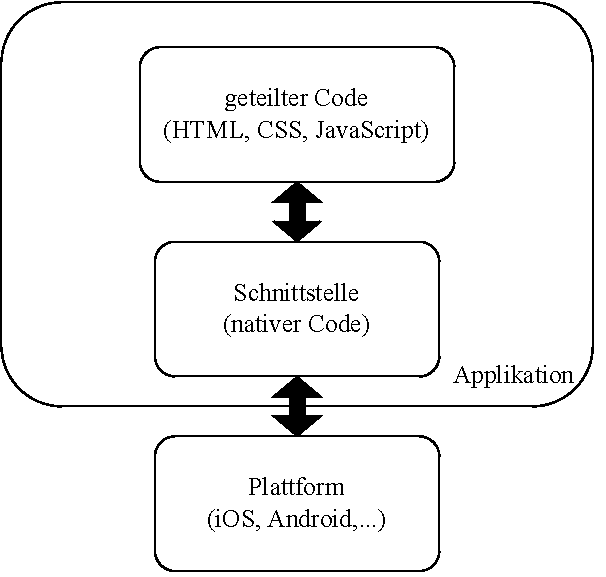
\includegraphics[height=9cm,keepaspectratio]{images/hybrid_architecture.drawio.pdf} 
  \caption{Architektur einer hybriden Applikationen}
  \label{fig:hybrid_architecture}
\end{figure}

Wie in Abbildung \ref{fig:hybrid_architecture} zu sehen ist, besteht diese Art von Applikation aus zwei Teilen.
Der erste Teil ist ein geteilter Code, der mit Web-Technologien erstellt wird und sowohl die UI als auch Applikationslogik enthält. Der geteilte Code kann dabei sowohl lokal als auch auf einem Server gespeichert werden und ist für mehrere Plattformen verwendbar \cite{2017hybrid_approach_end}.
Der zweite Teil formt eine Schnittstelle, die in nativen plattformspezifischen Code geschrieben ist. Der Schnittstellencode kann entweder selbstständig implementiert werden oder von einem Schnittstellen-Framework wie Cordova\footnote{\url{https://cordova.apache.org/}} zur Verfügung gestellt werden. Die Schnittstelle verwirklicht eine bidirektionale Kommunikation zwischen der Plattform und der Applikationslogik \cite{ELKASSAS2017163}. Somit kann die Anwendung auf die Funktionalitäten der Plattform zugreifen. Zusätzlich ermöglicht sie die Darstellung der Anwendung auf dem Endgerät. 

Grundsätzlich teilt dieser Ansatz die gleichen Vor- und Nachteile wie Web-Applikationen, da er zu einem großen Teil die selbe Technologien nutzt. Jedoch kann eine offline Funktionalität erreicht werden, wenn die Anwendung lokal gespeichert ist. Zusätzlich erhält die Applikation durch die Schnittstelle Zugriff auf die native Funktionalität und kann auf dem Gerät installiert werden. Weiterhin kann der geteilte Code sowohl auf den verschiedenen Plattformen, als auch in anderen Technologien wiederverwendet werden, da es sich im Prinzip um eine Webseite innerhalb einer Applikation handelt \cite{IEEE_development_classes}. Jedoch entsteht durch den zusätzlichen Web-Container, der geladen werden muss, um die UI anzuzeigen, eine erhöhte Ladezeit, die sich negativ auf die Performance der Applikation auswirkt \cite{IEEE_development_classes}.

\subsection{Interpretierte Applikationen}
\label{cha:3_2_interpretiert}
Bei interpretieren Cross-Plattform Anwendungen schreibt der Entwickler Code, der anschließend mithilfe eines Interpreters während der Laufzeit in ausführbaren Code übersetzt wird. Folglich besteht die auf dem Gerät installierte Anwendung aus zwei Teilen. Einerseits einem nativen Teil, oftmals Frameworkcode, der zum Übersetzen der eigentlichen Anwendung benötigt wird. Andererseits einem Cross-Plattform Teil, der die Anwendungslogik realisiert \cite{IEEE_development_classes}.

Der Unterschied zu einer hybriden Applikation besteht darin, dass die Anwendungen je nach Plattform anders aussehen können. So wird etwa die Benutzeroberfläche erst während der Laufzeit in eine native UI, mit den plattformspezifischen UI Elementen, übersetzt.
Dadurch wird eine Nutzung von nativen Elementen möglich, obwohl die Anwendung eigentlich in einer anderen Sprache definiert ist \cite{IEEE_development_classes}. 
Dazu kommt, dass eine Anwendungen auf allen Plattformen ausgeführt werden kann, die von dem entsprechenden Interpreter unterstützt wird \cite{server_side}.

Jedoch ergibt sich hierbei eine Abhängigkeit zum Framework und dessen unterstützten Plattformen. Zudem hat, durch die Interpretierung während der Laufzeit, dieser Ansatz eine hohe Reaktionszeit, da jede Zeile vor Ausführung erst durch den Interpreter übersetzt werden muss und somit eine extra Latenz zwischen jedem einzelnen Aufruf und dessen Ausführung entsteht \cite{server_side}.

\subsection{Cross-kompilierte Applikationen}
Bei cross-kompilierten Applikationen wird während der Entwicklung ebenfalls lediglich ein Quellcode geschrieben, jedoch wird dieser bereits vor Verteilung in nativen Code übersetzt. Daher muss der Übersetzungsprozess nur einmalig durchgeführt werden und nicht wie bei dem interpretierten Ansatz, bei jeder Benutzung. Um dies zu erreichen, wird ein Cross-Compiler benötigt, der für mehrere unterschiedliche Plattformen Kompilate erzeugt \cite{mobiledraft_cross_plattform}. Somit kann aus einem Code für jede Plattform eine eigene Anwendung gebaut werden, die ausschließlich aus nativem Code besteht und sich folglich für das Betriebssystem nicht von einer nativen Anwendung unterscheidet \cite{IEEE_development_classes}.Im Vergleich zur interpretieren Anwendung kann außerdem die App-Größe reduziert werden, da kein zusätzlicher Übersetzer benötigt wird \cite{mobiledraft_cross_plattform}.

Auch bei diesem Ansatz ist die Funktionalität und die Zahl der unterstützten Plattformen von dem genutzten Cross-Compiler abhängig. Einige dieser Frameworks nutzen eine spezialisierte Programmiersprache, sodass eine Wiederverwendung des Codes für einen anderen Ansatz erschwert wird. So wird etwa bei Flutter\footnote{\url{https://flutter.dev/}} die Sprache Dart\footnote{\url{https://dart.dev/}} genutzt.

\subsection{Gemischter Ansatz}
Die Entwicklungsansätze sollen in dieser Arbeit um einen weiteren Ansatz erweitert werden, wie ihn Khachouch et al \cite{IEEE_Khackouch_Al} in ihrer Arbeit aufführen. Sie definieren einen gemischten Ansatz, um die verschiedenen Ansätze kombinieren zu können. Somit können die Vorteile unterschiedlicher Ansätze vereint werden.


\section{Themenabgrenzung}
In dieser Arbeit sollen nicht die verschiedenen Programmiersprachen oder Frameworks innerhalb der einzelnen Ansätze verglichen werden, sondern viel mehr die Ansätze gegenseitig. Daher wird für eine Cross-Plattform Implementierung das Framework Flutter\footnote{https://flutter.dev/} genutzt, da dies das aktuell am meisten genutzte Framework\cite{statist_CP_Framework} ist und somit einen guten Repräsentanten für diese Gruppe darstellt. Für die Android Implementierungen wurde als Programmiersprache Kotlin\footnote{https://kotlinlang.org/} genutzt. 

Die nativen Implementierungen werden in dieser Arbeit auf eine Android Implementierung beschränkt. 
Einerseits sind iOS und Android vergleichbar, da beide nativ auf die vollständigen Funktionalitäten der Betriebssysteme zugreifen.
Dabei sind es nicht die verschiedenen Programmiersprachen und ihre Kleinigkeiten die entscheidend sind, um native Apps zu entwickeln, sondern die Konzepte.
So sagen Goadrich et al \cite{iOSvsAndroid} in einer Untersuchung, welche Plattform für einen Universitätskurs passend wäre, dass beide Umgebungen die für den Kurs benötigten Funktionalität haben.
Weiter sagen sie, dass Studenten dadurch praktische Erfahrung in der Applikationsentwicklung bekommen würden. Sie kommen am Ende auf den Schluss, dass es kein Unterschied macht welche Plattform dabei behandelt werden würde und beide Plattformen helfen, eine Grundlage zur Lehre der Grundideen für mobile Endgeräte Programmierung bilden würden.
Auch in Sachen Performance gibt es zwischen den Plattformen keine größere Unterschiede. So zeigt eine Untersuchung von Győrödi et al \cite{Android_IOS_Performance_comparison}, dass es zwar kleinere Unterschiede in der Performance gibt, es aber keine Plattform gibt, die insgesamt gesehen besser ist, als die andere.
Desweiteren stellt Android die deutlich größere Nutzergruppe dar. So besagen aktuelle Statistiken, dass Android aktuell einen Marktanteil von etwa 70\% hat, während iOS nur auf 30\% kommt \cite{statist_OS_worldwide}.  

Die betrachteten Implementierungen umfassen ebenfalls keine Spieleimplementierung. Diese stellen zwar einen signifikanten Teil der in den Appstores vorhandenen Anwendungen dar, jedoch sind dies keine typischen Apps die von Appagenturen oder privaten Entwicklern produziert werden, sondern eher von Unternehmen mit Grafik- oder Spieleentwicklungshintergrund. Außerdem werden die meisten Apps nicht in Kotlin oder Swift direkt entwickelt, sondern mit Game- und Grafikprogrammen wie Unity oder ähnlichem gebaut. 



Der Schwerpunkt der Arbeit liegt außerdem auf Smartphone-Applikationen. Zwar sind in der Klasse der mobilen Endgeräte auch Laptops mit den Betriebssystemen Windows, MacOS oder die verschiedenen Linux distributionen, dennoch werden Applikationen primär für den Smartphone Markt entwickelt, während für mobile Rechner dann eher ein Programm schreibt.
\TODO{Warum auf Smartphone bei Untersuchung beschränkt?}

%To think if to remove
\section{Projektbeschreibung}
Als Basis für diese Arbeit wird eine bereits bestehende Elixir-Web-Anwendung genutzt. Hierbei handelt  es sich um eine Plattform, die das Ziel hat, das Verleihen und Leihen innerhalb von Bekanntschaftskreisen zu vereinfachen/ ermöglichen. Hierfür kann jeder Nutzer seine eigenen, verleihbaren Gegenstände auf der Plattform eintragen. Zusätzlich können Nutzer sogenannte Kreise erstellen und zusammen mit Freunden bzw. Familie beitreten. Jeder kann dann die Gegenstände sehen, die in den verschiedenen Kreisen vorhanden sind, in denen er Mitglied ist. Zur Kontaktaufnahme gibt es ein Chatsystem, bei dem sich Leute Nachrichten hin und her schicken können, um den Austausch zu organisieren. Zur Kommunikation mit einer Applikation besitzt das System eine GraphQL-Schnittstelle, über die alle benötigten Daten abgefragt werden können. Auch kann der Nutzer über die Schnittstelle authentifiziert werden und neue Nachrichten versendet.

\section{Funktionsumfang der Beispiel-Anwendung}
Damit die abgebildete Anwendung ein gutes Beispiel für eine Applikationsentwicklung darstellt, wurde beim Entwurf des Funktionsumfangs darauf geachtet, möglichst viele der typischen Funktionalitäten von Applikationen abzudecken. Eine Befragung \cite{JetBrains_miscellaneous_2021} mobiler Anwendungsentwickler durch JetBrains ergab, dass die wichtigsten Funktionen Datenspeicherung, Kommunikation über Netzwerk, Medienanzeige, Statusmanagement, Navigation, Datensynchronisierung, Dateien lesen/schreiben sind.
Das in der Arbeit betrachtete Projekt beschränkt sich dabei auf folgende Funktionalitäten:

Es soll eine App gebaut werden, die sich an der bestehende Web-Anwendung orientiert und einen Teil der Funktionalität durch die Programmierung abbildet. Dabei können die Implementierungen in zwei Gruppen unterteilt werden, die im Folgenden genauer beschrieben werden.

\subsubsection{Funktionalität mit Applikationscode}
Bei der nativen und der cross-kompilierten Applikation wird die komplette Funktionalität innerhalb der implementierten Applikation abgebildet. Die Verbindungen zwischen den umgesetzten Benutzeroberflächen ist in Abbildung \ref{fig:pageflow} dargestellt. Dabei sind Pfeile mit flacher Spitze Weiterleitungen die automatisch passieren und Pfeile ohne eine Beschriftung Abläufe, die durch das Drücken eines Buttons implementiert sind. Außerdem entsprechen die Zustände in der Abbildung den einzelnen Seiten der Anwendung. Diese sind eine Start-, Login-, Profil-, Kommunikations- und eine Chatseite. Dadurch können die oben genannte Aspekte vollständig abgedeckt werden. So ist etwa durch den Login das Statusmanagment und die Kommunikation über ein Netzwerk implementiert. 

\begin{figure}[ht]
  \centering
  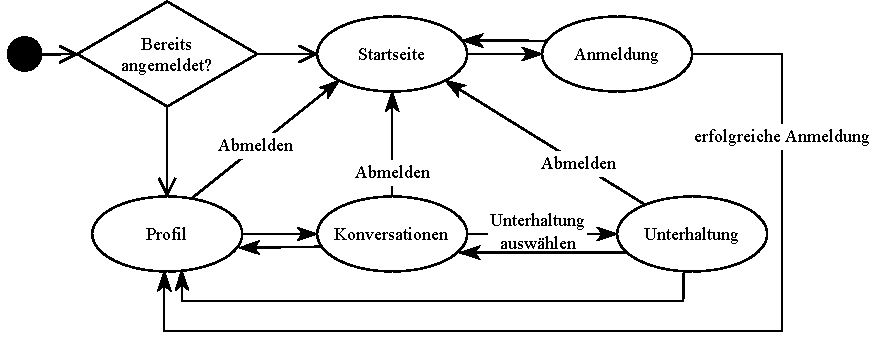
\includegraphics[height=7cm,keepaspectratio]{images/Pageflow_native_flutter.drawio.pdf} 
  \caption[Seitenablauf der implemierten nativen und cross-kompilierten Applikation]{Verbindungen zwischen den Seiten der implementierten Applikation des nativen und des cross-kompilierten Ansatzes}
  \label{fig:pageflow}
\end{figure}

Der Nutzer verwendet die Anwendung, wie im Folgenden beschrieben. Zunächst wird die App geöffnet. Wenn der Nutzer nicht eingeloggt ist, landet er auf einer Startseite/Willkommensseite, von welcher aus er sich einloggen kann. Ist er jedoch angemeldet, so wird er automatisch auf die Profil Seite weitergeleitet, auf der von einem Server geladene Daten angezeigt werden. Er kann außerdem auf das integrierte Chatsystem zugreifen und auch neue Nachrichten an andere Nutzer verschicken. Von allen Seiten mit benötigter Authentifizierung, gelangt der Nutzer durch Abmelden wieder auf die Startseite.

\subsubsection{Funktionalität mit Web-Integrierung}
In dieser Gruppe wird ein Teil oder auch die komplette Applikationslogik durch das Einbinden der Web-Anwendung in die Applikation ersetzt. So wird bei der Implementierung des hybriden Ansatzes die bereits existierende Website in eine native programmierte Applikation eingebunden. Der Applikationscode übernimmt dabei die Aufgaben, die klassischer Weise durch ein Framework erfüllt werden würde. Sie ist jedoch durch die spezifische Implementierung der Webseite stark in der Funktionalität eingeschränkt.

Bei der gemischten   Implementierung wird zwischen der Web-Anwendung und Benutzeroberflächen, die mit dem Cross-Compiler Framework Flutter erstellt wurden, gewechselt. Dabei werden insbesondere der Login, die Profilseite und das Chat System durch Flutter Seiten ersetzt, während der Rest der Anwendung durch die Web-Anwendung dargestellt wird. Daher ist dieser Ansatz eine Mischung aus dem hybriden und dem cross-kompilierten Ansatz.



\chapter{Entwicklung}
In diesem Kapitel werden die vier verschiedene Implementierungen erklärt. Dabei wird zu jedem Ansatz einige Grundlagen, genutzte externe Bibliotheken, Herausforderungen und ein Fazit zu der Implementierung vorgestellt. Dadurch sollen die Implementierungen reproduzierbar und Erkenntnisse während der Entwicklung geteilt werden.
\section{Entwicklung Nativer Android Applikation}
Die native Entwicklung ist die ursprünglichste von allen Arten. Android etwa wurde 2008 vorgestellt. 
Damals wurden die Apps für Android noch in Java entwickelt, eine Sprache die in der Anwendungsentwicklung damals und heute noch sehr gut bekannt ist und auch oft noch als Programmiersprachen an den Universitäten gelehrt wird. 
2019 jedoch änderte Google die offiziell bevorzugte Programmiersprache zu Kotlin. 
Kotlin ist von Jetbrains entwickelt um einen Ersatz für Java zu finden. 
Sie entwickelten eine Sprache die alle benötigten Funktionen für eine effektive Appentwicklung hat, jedoch genauso schnell kompiliert werden kann. 
Eine ähnliche Entwicklung fand auch bei Apple statt, die in Folge dessen von Objectiv-C zu Swift wechselten. 
Durch die Entwicklung eigener Sprachen haben sie die Kontrolle was in den Sprachen passiert und können diese perfekt für ihre Bedürfnisse anpassen.

Im folgenden wird die Implementierung eine native Android Applikation betrachtet werden.

\subsection{Grundlagen}

Die Entwicklung einer nativen Android \acp{App} besteht aus zwei separaten Teilen, Der erste Teil ist das Layout. Dabei wird ein Design für die Seite und eventuelle Elemente mit Hilfe der XML-Notation erstellt.
In der XML Datei wird ähnlich zu einer HTML Seite, die Oberfläche aufgebaut. Als Wurzelelement einer Seite ist ein Layoutelement. Neben einem linearem Layout oder einem Tabellenlayout, gibt es hier vor allem das so genannte \verb|Constraint-Layout|\footnote{https://developer.android.com/guide/topics/large-screens/support-different-screen-sizes}. 
Es ist das wichtigste Layout in Android, da wie der Name bereits andeutet, die Positionen der Elemente abhängig von anderen Elementen definiert ist. Durch diese Eigenschaft, eignet es sich besonders gut, um Designs für unterschiedliche Bildschirmgrößen zu erstellen. Es bietet dabei nicht nur die Möglichkeit, die Position, sondern auch die Größe abhängig davon zu definieren. Grundsätzlich hat Android nur zwei Optionen um die Größe eines Elements zu definieren. Es kann die größe des umgebenden Elements annehmen oder eine eindeutig definierte Größe. Durch das \verb|Constraint-Layout| kann jedoch über die Abhängigkeit zu beiden Seiten einer Richtung dazu gebracht werden, den verfügbaren Platz auszufüllen.

Der zweite Teil der Implementierung ist die Logik. Sie ist dabei in drei Klassen unterteilt. 
Die erste Klasse, die sogenannte Activity ist die Hauptklasse für eine Seite. In ihr wird alles gesteuert. Das Layout wird aufgerufen und der aktuellen Seite hinzugefügt, es werden alle Funktionalitäten zu den Elementen der Benutzeroberfläche hinzugefügt und ordnet der Oberfläche die Daten und den Listen ihre separaten Controller zu.

Dies ist ebenfalls die zweite Klasse. ListAdapter sind die Controller Klassen für Listen in Android. Listen werden dabei mit Elementen gebaut , die wiederverwendet werden, sobald sie außerhalb des Sichtfeldes sind. Dafür benötigt jede Liste einen Adapter, der dafür verantwortlich ist, die richtigen Elemente auszuwählen und Funktionalität und Daten hinzuzufügen.

Die dritte Klasse sind ViewModels\footnote{https://developer.android.com/topic/libraries/architecture/viewmodel}. Diese sind die Schnittstelle zwischen der Datenhaltung und der Activity. In einem ViewModel werden Daten abgefragt und Daten zwischengespeichert, die eine Konfigurationsänderung überstehen sollen. Diese sind etwa eine Änderung der Orientierung des Gerätes. Dies ist möglich, da ViewModels erst beendet werden, wenn ihre zugeordnete Aktivität final beendet wird. 
Durch die Nutzung kann die Performance verbessert werden. Es werden unnötige mehrfach Abfragen von Daten verhindert. Dazu kommt, dass ViewModels auf einem anderen Thread laufen als die Activity. Dadurch kann diese Events der \ac{UI} abfangen und weiterhin reagieren, während das ViewModel die nötige Daten sammelt.


\subsection{Genutzte Bibliotheken}
Die erste Bibliothek, die zur GraphQl-Kommunikation gewählt wurde, ist Apollo Kotlin. 
\TODO{Nochmal überlegen wegen dem wörtlichen Zitat}
"Apollo Kotlin ist ein GraphQL Client, der Kotlin und Java Modelle von GraphQL Queries erzeugt."\cite{Apollo_kotlin_docs} 
Anfänglich wird eine Konfigurationsdatei erstellt, in der Sachen wie der GraphQL-Endpunkt definiert werden. 
Danach stellt der Client eine Verbindung zu der GraphQL-\ac{API} her und fragt die Schnittstellendefinition ab, die im Anschluss gespeichert werden. 
Danach können die einzelnen GraphQL Befehle in einzelne Datein geschrieben werden. Aus diesen werden dann Modelle erstellt, die wie einfache Klassen im Applikationscode aufgerufen werden können.
Da Apollo die genaue Schnittstellendefinition hat, erzeugt es automatisch aus der \ac{JSON} Antwort des Servers ein Antwortobjekt und ordnet den einzelnen Stufen der Antwort die jeweiligen Datentypen zu.
Der Client wird der Applikation als globales Attribut hinzugefügt. Dadurch haben alle Activities darauf Zugriff und er kann einfach global geändert werden , wenn der Authentifizierungsstatus geändert wird.

Die zweite wichtige Bibliothek die genutzt wird, ist Room\footnote{https://developer.android.com/training/data-storage/room}. Sie ist Teil von Android Jetpack, dass ein Set an Bibliotheken ist, dass helfen soll, einfach und sauber Apps zu bauen, die über die verschiedenen Android-Versionen hinweg funktionieren \cite{Jetpack_android}. Room selber ist dabei der Teil, der es ermöglichen soll einen möglichst effizienten Datenbank Zugriff zu haben. 
Die Besonderheit ist, dass Room eine Zwischenebene darstellt, die sowohl die geschriebenen SQL Befehle überprüft und validiert, die asynchronität der Datenbankoperationen vereinfacht und durch Annotation redundanten Code verhindert \cite{Room_docs}.

Zum Speichern des Authentifizierungsstrings wurden sogenannte Shared-Preferences\footnote{https://developer.android.com/reference/android/content/SharedPreferences} genutzt. Sie sind ein weiterer Teil von Android Jetpack. Sie werden genutzt, um Key-Value Werte ohne großen Aufwand innerhalb der Applikation zu speichern. Sie können von innerhalb der ganzen Applikation abgefragt hinzugefügt, geändert oder gelöscht werden. Hierfür muss keine eigene Entität in der Datenbank angelegt werden und der Zugriff ist schneller. Sie sind jedoch nur für einfache Daten geeignet, da lediglich primitive Datentypen genutzt werden können. Daher werden sie vor allem für Werte wie Authentifizierung oder bestimmte Flags geeignet um den Status der App zu bestimmen.


\subsection{Fazit Android Nativ}
Nativ hat einige Vorteile. Es ist ein gut dokumentierter Ansatz, für den es für fast alle Probleme eine erprobte und funktionierende Lösung gibt. So war das Finden einer passenden GraphQL Bibliothek eine Leichtigkeit, da Apollo in diesem Bereich für Kotlin als Standardbibliothek gilt. Dazu kommt, dass es viele Bibliotheken gibt, die Google/JetBrains selber anbieten, um die Entwicklung von Apps zu vereinfachen und zu standardisieren.

Ein Vorteil der Layoutentwicklung in diesem Bereich ist, dass man das Layout in einer sofortigen Anzeige zusammenbauen kann und somit immer sofort sehen kann wie es aussieht. Jedoch ist dies eine Anzeige die nur die Oberfläche ohne Funktionalität oder von der Activity hinzugefügte Daten anzeigt. Wenn also hier Änderungen betrachtet oder getestet werden sollen, so muss die App neugebaut werden. Neben der Zeit, die es dauert die Änderungen zu laden, startet die App außerdem wieder vom Startbildschirm. Dadurch wird der Entwicklungsprozess verlangsamt und erschwert,


\section{Entwicklung einer hybriden Android Applikation mittels eines WebView-Containers}
Der zweite realisierte Ansatz ist eine hybride Applikation, die mit Kotlin implementiert wurde. 
Da einerseits die Implementierung der Web-Komponente durch viele verschiedene Ansätze umgesetzt werden kann und andererseits in diesem Fall bereits eine Webseite existiert, wird folglich nur auf die Implementierung der Schnittstelle eingegangen. 
Um ein besseres Verständnis über die Funktionalität des hybriden Ansatzes zu erhalten, wird auf die Nutzung eines Frameworks verzichtet und die Schnittstelle zwischen der eingebundenen Webseite und der Plattform nativ entwickelt.
Dabei wird die grundlegende Funktionalität ermöglicht. Eine umfänglichere Nutzung von Plattformfunktionalität wird in einem Exkurs vorgestellt.

\subsection{Grundlagen}
Um eine Minimalversion zu erhalten, wird eine native Applikation benötigt, die eine WebView-Komponente\footnote{https://developer.android.com/reference/android/webkit/WebView} enthält. Um die Funktionalität der Webseite zu ermöglichen, müssen unter Anderem die folgenden Aspekte beachtet werden.

So benutzen rund 98\% aller Webseiten JavaScript in ihrem Code, um zum Beispiel ein Menü ein oder auszublenden, ohne die Seite neu laden zu müssen \footnote{https://w3techs.com/technologies/details/cp-javascript}. 
Dazu muss jedoch JavaScript in der WebView aktiviert werden. 
Jedoch kann die Aktivierung von JavaScript ein Sicherheitsrisiko darstellen. So können etwa fremde Webseiten ebenfalls versuchen, auf das Gerät zuzugreifen \cite{webview_javascript_security}. 
Daher sollte die Implementierung externe Links erkennen und diese in einem externen Browser-Fenster öffnen.
Die Links können dabei entweder in dem normalen Browser des Gerätes geöffnet werden oder in einem CustomTabsIntent\footnote{https://developer.android.com/reference/androidx/browser/customtabs/CustomTabsIntent}.
Dadurch entsteht ein Browsertab in der eigenen Applikation, dass etwa in der Akzentfarbe der Applikation angepasst werden kann um eine Zugehörigkeit erkennbar zu machen, jedoch dennoch einen externen Browser zu erhalten. Es ist jedoch durch die angezeigte Funktionsleiste mit angezeigter URL am oberen Bildschirmrand dennoch als externer Inhalt erkennbar.

Um dies zu ermöglichen muss jedoch die aufgerufene URL abgefangen werden und entschieden werden, wie mit der aufgerufenen URL verfahren werden soll. So ist eine einfache Grundkonfiguration, dass alle URLs die zur angezeigten Webapplikation gehören zugelassen werden, während externe Links weitergeleitet werden.

Eine letzte Konfiguration, die benötigt wird um etwa das Login mit Google zu ermöglichen ist das Setzen eines UserAgentStrings. Er ist eine Text Flagge, die in einem HTTP-Paket zu finden ist. Sie beinhaltet Informationen zu dem benutzten Client oder der genutzten Hardware. Außerdem wird sie auch genutzt, um verdächtige Pakete heraus zu filtern\cite{UserAgentString}. So filtert Google LogIn-Anfragen herraus, bei denen der UserAgent nicht gesetzt ist. Dieser kann durch das Setzen der Variable auf dem Webcontainer definiert werden.

Mit diesen Konfigurationen ist eine grundsätzliche Funktionalität einer Webapplikation sichergestellt. So kann an diesem Punkt theoretisch eine erste Version veröffentlicht werden. Jedoch ist an diesem Punkt dem Nutzer immer noch sichtbar, dass es sich bei dem Inhalt um eine Webseite handelt. Um dies zu verhindern können über die Layoutdatei native Elemente über oder um das WebView anlegen. So kann etwa ein Home Button dem Layout hinzugefügt werden, um der Anzeige native Elemente hinzuzufügen.

Neben der Konfiguration des Aussehens kann die WebApplikation noch in der benutzung von Gerätefunktionalität angepasst werden. Auf eine derartige mögliche Erweiterung soll deswegen im Folgenden Exkurs etwas eingegangen werden.

\subsection{Exkurs: Nutzung von Plattformfunktionalität}
Wie in Kapitel \ref{cha:3_hybrid} erwähnt, haben hybride Applikationen die Möglichkeit auf Plattformfunktionalität zuzugreifen. Dies ist der Teil, den Frameworks typischer Weise bereits umgesetzt haben und um die ein Entwickler sich normalerweise keine Gedanken machen muss. Jedoch wird in dieser Arbeit kein Framework genutzt, um einen Möglichen Ansatz zu zeigen, dies in die eigene Applikation zu integrieren. So kann ein von der App initialisiertes und der WebView hinzugefügtes WebAppInterface\footnote{https://developer.android.com/guide/webapps/webview\#BindingJavaScript} direkt aus dem JavaScript der Webseite aufgerufen werden \cite{webview_javascript_security}. Dafür werden Objekte und ihre öffentlichen Methoden dem Webcontainer unter einem definierten Namen zur Verfügung gestellt. Es können dabei sowohl Daten gesendet als auch empfangen werden.

Auch kann aus der Applikation JavaScript Code aufgerufen beziehungsweise ausgeführt werden. Dafür wird mit der loadUrl Methode, die in der WebView normalerweise einen Link aufruft, JavaScript-Code mit dem Präfix \verb|"javascript:"| der WebAnwendung hinzugefügt \cite{webview_javascript_security}. Dies kann sowohl selbst geschriebener Code als auch ein Aufruf bereits definierter Methoden sein. Dies zeigt jedoch, dass auch innerhalb der Webanwendung ein besonderes Augenmerk auf die Sicherheit gesetzt werden muss, da unter Umständen neben der Applikation, auch die Webseite angreifbar ist. So könnten bösartige Applikationen versuchen, über die JavaScript Schnittstelle eigenes JavaScript auszuführen, um so etwa den aufgerufenen Webserver zu attackieren. Dies ist möglich, da JavaScript-Code, der über loadUrl hinzugefügt wurde, im aktuell angezeigten Kontext gleichwertig wie von von der Webanwendung stammendes JavaScript ausgeführt wird \cite{webview_javascript_security},

\subsection{Fazit hybride Implementierung}
Ein Vorteil dieser Implementierung ist die Entwicklungsgeschwindigkeit, die erreicht werden kann, wenn bereits eine Webanwendung existiert. Anstatt die Anwendung komplett neu zu schreiben und somit multiple Implementierungen der Anwendungslogik zu erstellen, kann mit diesem Ansatz die Webanwendung in eine native Applikation eingebettet werden.
Ein weiterer Vorteil ist, dass durch die Nutzung der extern gehosteten Webanwendungen, Änderungen am Inhalt der angezeigten Anwendung nicht erst auf den Geräten der Nutzer installiert werden müssen, sondern direkt nach einem Neuladen der Webseite bei allen Nutzern verfügbar ist. 
Dazu kommt, dass an der eigentlichen Applikation nur sehr selten Änderungen durchgeführt werden müssen, da hier in den meisten Fällen nicht viel Logik verbaut ist.

Ein Nachteil ist, dass in diesem Fall die App nur nutzbar ist, wenn eine aktive Internetverbindung besteht, da der Großteil der angezeigten App, aus der Webseite bestehen. Dazu kommt, dass der Programmier- und Wartungsaufwand steigt, wenn eine umfangreiche Nutzung von Gerätefunktionalität geplant ist. Des Weiteren wird bei dieser Implementierungsart wieder eine eigene Implementierung des nativen Containers für jede Plattform benötigt., dies kann jedoch durch die Nutzung eines Frameworks verhindert werden. Ein Problem für diese Art der Entwicklung sind jedoch die Review Guidelines des Apple AppStores\footnote{https://developer.apple.com/app-store/review/guidelines/\#minimum-functionality}. Diese legen fest, dass die App nicht einfach nur ein Container für eine Webseite sein darf, sondern zu großen Teilen aus für den Nutzer nützlichen Funktionalitäten bestehen muss. Dadurch ist es wahrscheinlich, dass eine Implementierung im Umfang der hier dargestellten Applikation von Apple nicht veröffentlicht werden würde, wenn nicht noch zusätzliche Funktionalität hinzufügt wird.

Einige der Vor und Nachteile sind jedoch stark von der hier vorgestellten Implementierung abhängig. So wird etwa durch die Nutzung einer lokal gespeicherten Implementierung eine offline Funktionalität erreicht, jedoch müssen dadurch Änderungen über den normalen Updateprozess der einzelnen Plattformen verteilt werden.
Auch kann die gesamte Implementierung durch die Nutzung von Frameworks erledigt werden, jedoch muss die Webseite dann an dieses Framework angepasst werden und die nutzbare Funktionalität durch die implementierten Lösungen eingeschränkt sein. 


\section{Entwicklung Cross-Plattform Applikation mit Flutter}
Der dritte Ansatz der hier erklärt werden soll, ist eine Cross-Plattform-Implementierung mit Hilfe des Flutter Frameworks.

\subsection{Flutter Grundlagen}
Flutter ist ein 2017 von Google veröffentlichtes Framework das mittlerweile zum bedeutendsten Cross-Plattform-Framework geworden ist\cite{statist_CP_Framework}. Neben viel Aufmerksamkeit von Entwicklern haben auch Firmen großes Interesse an Flutter. So hat etwa die Firma hinter Ubuntu, Canonical, angekündigt, dass alle von ihnen entwickelten Anwendungen, in Flutter programmiert werden\cite{Ubuntu_Flutter}. Als Programmiersprache wird dabei Dart benutzt, die je nach Plattform, mit unterschiedlichen Compilern übersetzt wird,

Eine Grundlage von Flutter ist \verb|Composition over inheritance|. Dieses Konzept ist besonders gut sichtbar beim Aufbau der Nutzeroberfläche. Alles ist ein Widget. Bis auf die Geschäftslogik ist alles, wie etwa Gestenerkennung, Layouthelfer und tatsächlich Angezeigte Elemente ein Widget\cite{Thiele_2018}. Dabei werden Widgets baumartig verschachtelt, wobei die meisten Widgets wieder ein oder mehrere Kinderelemente haben, die ein Widget sind. In Abbildung \ref{fig:flutter_layout_tree} etwa ist der Widget-Baum einer Menüleiste zu sehen. Dabei sind Container Elemente, die um Widgets gebaut werden, um weitere Sachen wie Abstände oder anderes hinzufügen. Nur bei Widgets wie in diesem Fall etwa Text oder Icon, stoppt der Baum, da diese keine weiteren Kinder haben.

\begin{figure}[ht]
  \centering
  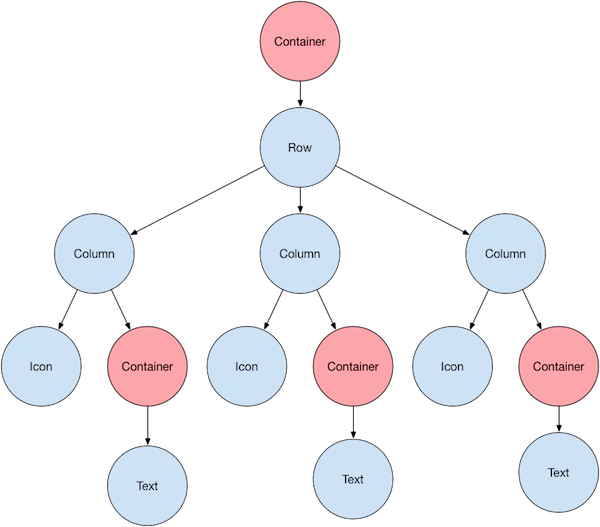
\includegraphics[height=7cm,keepaspectratio]{images/sample-flutter-layout.png} 
  \caption{Hierachie einer Menüleiste Quelle\protect\footnotemark}
  \label{fig:flutter_layout_tree}
\end{figure}

\footnotetext{https://docs.flutter.dev/development/ui/layout}

Anders als bei der nativen Implementierung wird in Flutter das Layoutfile mit der Funktionalität dahinter gemischt. Das bedeutet, dass die Funktionalität direkt beim definieren eines Knopfes zugeordnet wird. Dafür muss lediglich das Widget in den Baum eingefügt werden und danach das entsprechende Attribut gesetzt werden. Dadurch ist alles an einem Ort.

Da Flutter einen großen wert auf Perfomance legt, ist eine Änderung auf der \ac{UI} so gebaut, dass nur Elemente neu gebaut werden, die ihren Inhalt geändert haben. Dafür hat Flutter für \verb|Stateful Widgets|, die eine extra State Klasse besitzen. In diesem werden Daten gespeichert und sobald er sich ändert, registriert Flutter die Änderung und baut daraufhin das geänderte Widget und die in der Hierachie folgenden neu\cite{9623025}. Dadurch kann häufiges und vor allem vollständiges Neubauen des Widgetsbaums verhindert werden. Jedoch benötigt nicht jedes Element einen State. Wenn etwa bereits zum Zeitpunkt des Erzeugens des Widgets, alle Daten feststehen und auch nicht mehr geändert werden, dann wird kein State benötigt und es reicht ein \verb|Stateless Widget| für die Implementierung\cite[Kapitel~4]{Flutter_Recipes}. Dadurch wird einerseits die Implementierung eines States ersparrt und bei einem Neubau des Baums, kann das Widget-Element wieder genutzt werden und muss lediglich neu gerendert werden, was bei Flutter jedoch sehr performant ist.

Um sich wiederholenden Code zu sparen, kann in Flutter einfach ein eigene Widget geschrieben werden, dass im gesamten Projekt wie jedes andere Element auch, in den Widget-Tree eingefügt werden kann. Das Erstellen eines Widgets ist dabei der selbe Prozess wie das erstellen einer Seite. Es wird ein Knoten Element gewählt und dann mit anderen Elementen kombiniert, um die gewünschte Oberfläche zu erhalten. Außerdem muss entschieden werden, ob es ein Stateful oder Stateless Widget ist. Je nachdem muss noch ein zusätzlicher State implementiert werden.


\subsection{benutzte Plugins}
Das erste Plugin dass zu erwähnen ist, ist \verb|graphql\_flutter|\footnote{https://pub.dev/packages/graphql\_flutter}. Es ist ein Packet, dass ähnlich zu dem bereits erwähnten Apollo GraphQL einen Client zur Kommunikation mit einer GraphQL Schnittstelle. Damit der Client in allen Pages und Widgets verfügbar ist, muss die Konfiguration als Wurzel der Applikation gesetzt werden. Danach kann entweder über ein Widget oder über eine programmierte Funktion Die verschiedenen GraphQL Funktionen ausgeführt werden. Es ist ein Open Source von einer Community geschriebenes Plugin. Dies ist auch in der Nutzung spürbar. So sind einige Funktionalitäten nicht so sehr ausgereift wie bei der Apollo Implementierung. So muss etwa auf die einzelnen Felder der Antwort mit der JSON Zugriff \verb|Antwort.data[\"Feldname\"]|. Die Gefahr ist dabei hoch, dass durch ein Tippfehler der Zugriff schief läuft. Durch die Entwicklung von einer Community ist es allerdings einfacher Hilfe zu bekommen. So wurde während der Entwicklung ein paar Fragen auf dem dafür eingerichteten Discord-Server eingestellt, die professionell innerhalb einiger Stunden beantwortet wurden.

Das zweite wichtige Plugin ist Hive\footnote{https://pub.dev/packages/hive}. Es ist ein einfacher und schneller Key-Value Speicher, der Daten auhc über einen Neustart der App hinaus, in einer Datei innerhalb des Applikationsordner speichert. Er wird dafür genutzt, um den Identifikationsstring für den Server zu speichern. Es ist vergleichbar mit den \verb|SharedPreferences| der nativen Entwicklung vergleichbar, ist jedoch umfangreicher, da auch Objekte mit der richtigen Konfiguration gespeichert werden können und ist beim lesen vergleichbar beziehungsweise beim Schreiben schneller.

Ein drittes Plugin das hier noch erwähnt werden sollte ist \verb|simple\_gradient\_text|. Es ist ein Paket um ein Text mit Farbverlauf in der Schrift zu haben. Es ist also lediglich ein Paket, das zur Erstellung der Oberfläche genutzt wurde und ist dementsprechend hier nicht so wichtig. Jedoch zeigt sich hier wieder der Vorteil an einer aktiven Community. Bei der Installieren des Paketes gab es anfänglich einige Probleme, da es auf Android funktionierte aber auf anderen Plattformen nicht. Nach einer Unterhaltung mit dem Entwickler über ein erstelltes Problem auf GitHub ergab sich, dass das Plugin eine höhere Minimalversion von Dart benötigte, als in meiner Konfiguration eingestellt. Dadurch konnte bei mir der Fehler einfach behoben werden. Daraufhin wurde die Dokumentation des Paketes sowohl auf GitHub und dem zentralen Plugin Verzeichnis aktualisiert und um die entdeckte Anforderung erweitert.

Als letzte wichtige Bibliothek, wurde \verb|sqflite\_common\_ffi|\footnote{https://pub.dev/packages/sqflite\_common\_ffi} für die Implementierung der Datenbank genutzt. Es ist eine Bibliothek, dass auf Basis von \verb|sqlite3| eine Datenbankimplementierung für alle Plattformen anbietet.
Diese wird beim Start der Anwendung geöffnet und ist danach in der kompletten Anwendung verfügbar.
Mit ihre können alle gängigen \ac{CRUD}-Operationen durchgeführt werden. Die Implementierung ist dabei denkbar einfach.
Zum erstellen der Tabelle muss lediglich der SQL Befehl zum erstellen ausgeführt werden und danach kann über dedizierte \verb|insert| und \verb|query| Methoden die Daten gespeichert beziehungsweise abgefragt werden.
Nebenbei kann jede Art von SQL-Befehl ausgeführt werden, um Befehle auszuführen, die über die normale Implementierung hinaus gehen.


\subsection{Exkurs: Platform spezifische Funktionalität entwickeln}
Im Verlaufe der Entwicklung kann es vorkommen, dass eine gewisse Funktionalität, die essentiell für die Anwendung ist, bisher nicht implementiert wurde oder die Verfügbaren Bibliotheken nicht die gewünschte Funktionalität hat oder gewisse Plattformen nicht unterstützt werden. Für diesen Fall kann eigener Plattformcode geschrieben werden. Dafür wird einerseits der benötigte Dart Code geschrieben und dann der jeweilig notwendige Plattformcode. Zur Kommunikation zwischen den Verschiedenen Teilen werden dabei Plattform-Channels genutzt.\cite[Kapitel~12.3]{Flutter_Recipes}

Durch die Nutzung eines Kanals zur Kommunikation erlaubt es die Ausführung des Plattform Codes auf einem separaten Thread. Dadurch kann dieser asynchron ausgeführt werden und eine Blockade des Threads auf dem die \ac{UI} ausgeführt wird, verhindert werden\cite{plattform_code_flutter}.

Um weiteren Entwicklern die entwickelte Erweiterung zur Verfügung zu stellen kann außerdem das Plugin in das offizielle Repository von Flutter hochladen.

Es ist also möglich benötigte Funktionalität hinzuzufügen, solange sie auf den einzelnen Plattformen möglich ist. Jedoch werden für eine derartige Entwicklung das nötige Wissen benötigt, um den Plattformcode zu schreiben.

\subsection{Exkurs: Firebase}
Ein weiterer Aspekt, warum Flutter gerade bei kleineren App-Projekten gern genutzt wird, ist die umfangreiche Integrationsmöglichkeit von Firebase. Eine aktuelle Untersuchung ergab, dass in Android Applikationen die eine Analyse Software integriert haben, 92\% der weltweiten Applikationen, Firebase nutzt \cite{statist_analytics_SDK}.

Firebase ist eine Backend-as-a-service Lösung, die dabei helfen soll, schnell und einfach Anwendungen zu entwickeln und zu betreiben\footnote{https://firebase.google.com/}. Es ist also eine Sammlung von verschiedensten Tools und Plugins, die einem Entwickler die Möglichkeit geben soll, sich auf Design und Funktionalität der App konzentrieren zu können. Es umfasst Tools wie eben Analyse Software um Nutzungsdaten zu sammeln und zu analysieren, ein fertiges Chatsystem oder auch eine Cloud gestützte Datenbank Lösung. So schreiben Guzzi et Al, dass entweder ein Team an Entwickler angestellt werden müssten, das in monatelanger Arbeit ein Backend System programmieren würde, um dann eine Schnittstelle zu einem Backend zu bauen. Andererseits kann auch ein bereits bestehendes System gennommen werden. Mit Firebase werden tausende Zeilen Code eingespart und erhält dabei die Möglichkeit, asynchrone Aufrufe und nebenläufige Prozesse für eine reaktive App zu nutzen \cite[p.~608]{Flutter_Apprentice}.

Um eine Datenbank für seine App zu erstellen sind es wenige Schritte. So kann auf der Webseite von Firebase eine neue Datenbank angelegt werden. Danach wird die erzeugte Konfigurationsdateien für die jeweiligen Plattformen heruntergeladen. Diese werden den jeweiligen Implementierungen hinzugefügt. Danach müssen die Datenstrukturen lokal in der App entworfen werden und eine Verbindung hergestellt. Dafür werden die Daten-klasse mit JSON Konvertierungen, ein \ac{DAO} mit einer Methode zum speichern und holen der Daten und zuletzt noch einen Provider erzeugt. Außerdem besteht die Möglichkeit, neben einer online Datenbank ebenfalls eine offline Version hinzuzufügen, die synchronisiert wird, sobald eine Internetverbindung hergestellt wird \cite{Flutter_Apprentice}.

Ein weiterer Pluspunkt ist die Integration von Firebase-Authentifizierung. Es bietet eine fertige Lösung zur Authentifizierung von Nutzern. Es besteht außerdem die Möglichkeit, Benutzer zu kategorisieren beziehungsweise die Nutzung einzuschränken. So kann über Regeln in der Firebase-Website, präzise definiert werden, welcher Nutzer auf welche Daten zugreifen kann. Weiter können Nutzer auch von der Nutzung des Dienstes ausgeschlossen werden oder nur bestimmte Emailadressen zugelassen. Es bietet also ein vielseitig und umfangreiches Nutzerverwaltungstool \cite{Flutter_Apprentice}.

Firebase ist natürlich nicht nur für Flutter verfügbar, sondern genauso für die verschiedensten Programmiersprachen der Plattformen Android, iOS oder auch Web. Dennoch ist Flutter und Firebase ein interessantes Gesamtsystem. Denn durch Flutter muss lediglich einmal der Code zum Zugriff auf die Datenbak oder die anderen Dienste geschrieben werden. So wird nicht nur weiter Entwicklungszeit um sehr ähnlichen Code zu schreiben, sondern verhindert gleichzeitig eine unterschiedliche Definition der Entitäten oder anderen Elementen. Außerdem ist dadurch ein problemloser Wechsel von einem System zu einem anderen Möglich, da alle Anwendungen auf egal welcher Plattform gleich sind.

\subsection{Conclusion Flutter}
Durch die hier beschriebene Entwicklung kann mit Hilfe von einem Code, eine Anwendung geschrieben werden, die sowohl auf Android, iOS, Windows, Mac und Linux läuft. Lediglich die Web Implementierung funktioniert nicht, da der GraphQL Client hier keine richtige Verbindung erstellen kann. Für alle anderen Plattformen muss lediglich die Unterstützung deklariert, der Code in Plattform spezifischen Code compiliert und am Ende ausgeführt werden.

Das Tempo mit dem eine Flutter Anwendung entwickelt werden kann ist ähnlich wie eine einzelne native Implementierung. Dabei entsteht aber, wie bereits erwähnt, nicht nur die Implementierung für eine Plattform, sondern 5. Selbst wenn der Fokus der Entwicklung zuerst nur auf einer Plattform liegt, kann es sinnvoll sein Flutter zu nutzen um in Zukunft weitere Plattformen hinzuzufügen. Denn alle Plattformen können nachträglich noch exportiert werden.

Jedoch ist dies natürlich nicht immer möglich. Denn etwa der GraphQL Client ist nicht mit einer Web-Version kompatibel. Daher sollte bei der Wahl der Pakete darauf geachtet werden, welche Packete ausgewählt werden, um eine Inkompatibilität mit den gewünschten Plattformen zu verhindern. Wie bereits ausgeführt, kann versucht werden, solche Probleme durch eine eigene Implementierung zu lösen, dies ist jedoch mit einem erhöhten Aufwand und nötigen Wissen verbunden. Dabei ist die eigentliche Implementierung an sich nicht das eigentliche Problem, da auch hier dann native externe Bibliotheken genutzt werden können, jedoch ist die Konfiguration der Kommunikationsschnittstellen mitunter recht kompliziert und müssen sinnvoll implementiert sein, um die Performance nicht erheblich zu schwächen.

Flutter ist außerdem noch recht neu. So werden bei regelmäßigen Updates auch Änderungen eingeführt, die die Qualität und Entwicklung verbessern, jedoch dabei auch umfangreiche Änderungen in allen Applikationen notwendig macht. So wurde etwa ein Update veröffentlicht, dass das Nullsafety verbessern sollte. In Folge dessen musste jede Bibliothek angepasst und auch große Teile von Applikationen angepasst werden. Dadurch sind auch einige Anleitungen für Flutter veraltet und funktionieren in der aktuellsten Version nicht ohne Anpassungen.

Ein letzter Punkt ist, dass es keine Liste der verfügbaren Widgets innerhalb der Entwicklungsumgebung gibt. So muss alles, was nicht bereits bekannt ist gegoogelt werden. Hier wäre eine Übersicht über die typischen Elemente hilfreich um gerade für Anfänger den Einstieg zu erleichtern.

\section{Entwicklung einer gemischten Applikation mit WebView und Flutter}
Die vierte Implementierung ist dem gemischten Ansatz zuzuordnen. Sie besteht aus der Kombination einer hybriden Applikation und einer cross-kompilierten Applikation.
Hierbei sind die einzelnen Ansichten entweder eine mit Flutter implementierte Seite oder eine mittels WebView integrierte Ansicht der Webseite.
Durch diese Kombination soll die bereits bestehende Webseite wiederverwendet werden, während gleichzeitig bestimmte Teile des Systems für die mobile Nutzung angepasst werden und durch eigens programmierter Flutter Seiten ersetzt werden.
Dadurch kann ein Teil der Neuimplementierung vermieden werden, während die Nutzererfahrung für die neuen Plattformen optimiert werden kann.
Dabei soll weiterhin die Möglichkeit bestehen, die individuellen Applikationen aus einer gemeinsamen Code-Basis zu kompilieren.

\subsection{Grundlagen}
Da es sich wiederum um eine Flutter Applikation handelt gelten die selben Grundlagen wie in Kapitel \ref{cha:4_3_1}.
Zusätzlich wird nun eine WebView-Komponente hinzugefügt und zwischen Web-Oberflächen und Flutter-Seiten hin und her gewechselt.
Da dies kein weit verbreiteter Ansatz ist und es folglich keine offizielle Dokumentation oder Anleitungen für diesen Ansatz gibt, mussten hierzu einige Herausforderungen überwunden werden, die im Folgenden erläutert werden sollen.

Die Integration der Webseite ist ähnlich zum Vorgehen bei der hybriden Applikation. So werden aufgerufenen URLs abgefangen und es wird sich für eine von drei Vorgehensweisen entschieden. So werden Links zu externen Webseiten im Browser des Gerätes geöffnet. URL´s der eigenen Web-Anwendung, bei der die Web-Ansicht genutzt werden sollen, werden in der WebView geladen. Letztlich werden URL's, die zu Seiten gehören, die durch eine Flutter Seite angezeigt werden sollen, verworfen und die entsprechende Flutter Seite mit eventuell vorhandenen Parametern aus der URL geladen. 
Dementsprechend muss die Analyse und darauf folgende Unterscheidung der URLs deutlich feingradiger stattfinden.

Flutter beendet standardmäßig alle nicht mehr angezeigten Seiten und löscht dabei auch mögliche gespeicherte Informationen. So etwa auch die Navigationshistorie der WebView.
Da diese allerdings benötigt wird, um innerhalb der Webanwendung zurück zur vorherigen Seite zu navigieren, wird folglich eine Möglichkeit benötigt, um die Daten der WebView zu speichern. Dafür wurde das von Flutter bereitgestellte \verb|AutomaticKeepAliveMixin|\footnote{\url{https://api.flutter.dev/flutter/widgets/AutomaticKeepAliveClientMixin-mixin.html}} verwendet. 
Wie der Name beschreibt, werden damit die States von Widgets markiert, um zu bewirken, dass die Garbage Collection diesen nicht löscht. 
Bei einem erneuten Aufruf der Seite wird dann der noch vorhandene State geladen. Dadurch wird ein Zurücknavigieren in der Webseite auch nach dem vorherigen Verlassen der Web-Ansicht weiterhin möglich.

Es existiert außerdem bei diesem Ansatz eine zusätzliche Herausforderung bei der Navigation.
Dabei ist das Navigieren zu einer neuen Seite ohne Probleme durch die Navigation der WebView möglich. Die aufgerufene URLs werden abgefangen und ,wie bereits erklärt, weiterverarbeitet. Aus einer Flutter-Ansicht heraus wird dann entweder zu einer anderen Flutter-Ansicht navigiert oder die neue URL in der WebView aufgerufen. Bei der Rückwärtsnavigation ergibt sich jedoch folgendes Problem. Zwar kann die Flutter Navigation ohne Probleme von einer Flutter-Seite in die WebView zurückkehren, wo dann die Navigation der WebView übernimmt. Wurde jedoch in vorherigen Verlauf zu einer Flutter Webseite navigiert, so ist diese im Verlauf der Webseite enthalten. Da die Methode, welche über das weitere Verfahren der URL entscheidet, lediglich bei vorwärts navigieren aufgerufen wird, würde fälschlicher Weise die Webseite angezeigt werden und nicht die angepasste Flutter-Seite.
Um diese Herausforderung zu überwinden, wurden zwei mögliche Lösungen erarbeitet:
\begin{enumerate}
    \item Eine eigene Navigation programieren, in der genau definiert werden kann, wann eine URL als Webseite geladen wird und wann eine Flutter Seite aufgerufen wird. 
    \item Jedes mal, wenn von einer Flutter Seite zurück in eine WebView gewechselt wird, eine neue WebView erzeugen und somit den bereits vorhandenen Entscheidungsprozess für URLs nutzen. 
\end{enumerate}

Beide Lösungen haben Vor und Nachteile. So benötigt der erste Ansatz weniger Ressourcen, da lediglich eine WebView genutzt werden kann. Jedoch wird hier ein hoher Implementierungsaufwand benötigt, um eine angepasste Navigation zu schreiben. 
Beim zweiten Ansatz ist die Performance zwar schlechter, jedoch kann die von Flutter bereitgestellte Navigation genutzt werden. Somit können Fehler bei der Implementierung und ein zusätzlicher Programmieraufwand vermindert oder vermieden werden.
Wenn zusätzlich sinnvolle Punkte in der App definiert werden, an welchen die Navigationshistorie der Flutter-Navigation gelöscht wird, können folglich alte WebView Konfigurationen von der Garbage Collection gelöscht werden und folglich die vom Ansatz benötigten Ressourcen reduziert werden. Daher wurde für die Implementierung die zweite Lösung gewählt. 

Eine letzte Herausforderung war die Kombination der verschiedenen Technologien. Beispielsweise wurde bei der Web-Implementierung eine sogenannte Live-Komponente benutzt. Diese sorgt dafür, dass bei einem Wechsel von einer Seite zu einer anderen, keine neue URL geladen wird, sondern lediglich der Inhalt dynamisch nachgeladen wird. Dies lag zum Beispiel bei der Umsetzung des Chats vor. So war die Überssichtsseite der Konversationen mit der Anzeige der einzelnen Chats über diese Technologie verbunden. Deshalb konnte nicht ,wie ursprünglich geplant, lediglich die Chat-Seite durch Flutter ersetzt werden, sondern es musste auch die davorliegende Übersichtsseite umgesetzt werden.

\subsection{Benutzte Packages}
Es wurden die selben Erweiterungen wie in der Flutter Implementierung benutzt. Zusätzlich wurde ein WebView-Package benötigt, um die hybride Implementierung zu ermöglichen. Hierfür wird das von Flutter veröffentliche \verb|webview_flutter|\footnote{\url{https://pub.dev/packages/webview\_flutter}} Package genutzt. Anzumerken ist, dass die Wahl der richtigen Erweiterung kompliziert war, da keine der Optionen alle Plattformen unterstützte. Letztendlich wurde die offizielle Erweiterung gewählt, welche lediglich Android und iOS unterstützt.

\subsection{Fazit gemischte Implementierung}
Im Vergleich zur hybriden Implementierung ist mehr Implementierungsaufwand nötig, da Teile der Webseite durch eine eigene Implementierung ersetzt werden. Jedoch konnte die Benutzbarkeit der Applikation verbessert werden, da durch das gezielte Ersetzen der Webanwendung eine für die Plattform speziell angepasste Funktionalität oder Aussehen erreicht werden kann. Dabei kann Implementierungszeit im Vergleich zur nativen beziehungsweise cross-kompilierten Applikation gespart werden, wenn die Teile der Webanwendung, die von einem derartigen Umbau nicht profitieren, weiterhin als Webseite angezeigt werden.
Außerdem ermöglicht dieser Ansatz, dass ein Umbau von Webanwendung zu Applikation iterativ möglich ist und somit eine erste Version früher veröffentlicht werden kann.

Jedoch entstanden durch die Nutzung des gemischten Ansatzes einige Herausforderungen, für die es wenig Hilfestellungen in Foren oder Dokumentationen gibt. Daher ist dieser Ansatz mit einem erhöhten Aufwand verbunden und es besteht die Gefahr, dass etwa eine reine cross-kompilierte Implementierung schneller entwickelt werden könnte.
\chapter{Auswertung}
In dem folgenden Kapitel sollen die Ergebnisse der unterschiedlichen Implementierungen ausgewertet und analysiert werden. Dafür werden einige ausgewählte Kriterien anhand der Implementierungen und weiteren Quellen bestimmt und anschließend analysiert.

\section{Performance und Entwicklung}
Ein wichtiger Faktor bei der Entwicklung einer Applikation ist die Applikations-Performance. Da diese die Erfahrung bei der Benutzung beeinflusst, sollten Apps möglichst performant laufen, um die Ressourcen des Gerätes zu schonen und eine flüssige UI zu garantieren. Außerdem benötigen Entwickler einen einfachen und zeitsparenden Ablauf für typische Entwicklungsoperationen, wie etwa das anfängliche Kompilieren, oder das Laden von Änderungen. Auch die Möglichkeiten des Debuggen und Testens spielen bei der Entwicklung eine Rolle. Diese Faktoren sollen im Folgenden analysiert werden.

\subsubsection{Performance}

\begin{table}[ht]
\centering
\caption{Performancemessung der verschiedenen Applikationen}
\begin{tabular}{ |p{4cm}||p{3cm}|p{2.5cm}|p{2.5cm}|p{2.5cm}|p{2.5cm}| }
 \hline
 Parameter & gemischte Applikation & cross-kompilierte Applikation & native Applikation & hybride Applikation \\
 \hline
 Durchschnittliche CPU-Auslastung       &   2,54\%&   1,96\%& 0,9\%& 1,8\%\\
  \hline
 Maximale CPU- Auslastung  & 9,8\%& 6,4\%& 3,6\%& 7,4\%\\
  \hline
 Durchschnittliche RAM-Auslastung & 215,38 MB& 150,68MB& 86,74MB& 107,68MB\\
  \hline
 Maximale RAM- Auslastung & 238,00MB& 175,46MB& 100,64MB& 117,06MB\\
  \hline
 App-Größe & 7,4MB& 7,2MB& 5,2MB& 4,4MB\\
  \hline
 Maximale Startzeit & 532ms& 452ms& 263ms& 486ms\\
 \hline
 Durchschnittliche Renderzeit &8,68ms& 5,12ms& 9,04ms& 21,88ms\\
 \hline
\end{tabular}
\label{tab:evaluations_performance}
\end{table}
\newpage
In Tabelle \ref{tab:evaluations_performance} sind die Ergebnisse der Performance-Messungen zu sehen, die an den in Kapitel \ref{cha:4_Entwicklung} beschriebenen Implementierungen durchgeführt wurden. Dabei wurde die durchschnittliche und maximale Auslastung der CPU und des RAMs, sowie die App-Größe, maximale Startzeit der Applikation und die durchschnittliche Renderzeit gemessen. 
Die Renderzeit entspricht dabei der Zeit, die benötigt wird, bis eine Änderungen der Benutzeroberfläche, fertig verarbeitet, angezeigt werden kann.

Die Messungen wurden mit dem Programm Apptim\footnote{\url{https://www.apptim.com/}} durchgeführt. Dieses zeichnet die Performance von Applikationen während der Ausführung auf einem verbundenen Gerät auf. Die Tests wurden mit einem Google Pixel 5 durchgeführt, welches mit Android 12 beziehungsweise API Level 31 läuft. Es hat dabei 8GB DDR4-RAM und eine 8-Kern-CPU, die mit durchschnittlich 1,9 GHz getaktet ist.
Der Test wurde dabei für jede Implementierung fünf mal wiederholt und am Ende aus den Ergebnissen ein Durchschnittswert gebildet.
Die Apps wurden nach jeder Nutzung zurückgesetzt und alle anderen Applikationen wurden während der Tests beendet.
Zusätzlich wurde jeweils die Release-Version der Applikationen installiert, so dass die Performance gemessen wird, die auch ein Nutzer tatsächlich erleben würde.

Hierbei ist erkennbar, dass die native Implementierung insgesamt die performanteste ist und dabei in etwa die Hälfte der Auslastung erreicht, wi e die cross-kompilierte Applikation benötigt.
Dahingegen hat die gemischte App im Vergleich die höchste Auslastung und benötigt die längste Startzeit.
Nach Programmiersprachen betrachtet, haben die mit Dart programmierten Flutter Applikationen die geringste Renderzeit, während sie jedoch mehr RAM benötigen als die mit Kotlin implementierten Applikationen.
Die Implementierungen mit einem Web-Container, also die Hybride und Gemischte, verschlechtern sich im Vergleich zu den anderen beiden Implementierungen in der Performance deutlich. Daraus lässt sich schließen, dass ein Web-Container eine  Performanceverschlechterung verursacht. So ist etwa die hybride Applikation in den Messwerten ähnlich zu der cross-kompilierten Applikation, obwohl sie lediglich einen Web-Container ausführt und anzeigt, während die Flutter App hingegen die komplette Benutzeroberfläche und Kommunikation mit dem Server ausführt. Dies ist auch in der deutlich geringeren App-Größe der hybriden-Applikation zu erkennen.  

Die geringere Renderzeit der Flutter Applikationen ist insofern unerwartet, da Flutter die Applikation in nativen Code übersetzt und somit eine ähnliche bis schlechtere Leistung zu erwarten wäre. Jedoch nutzt Flutter für die UI keinen nativen Code, sondern eine eigene Grafikbibliothek namens Skia\footnote{\url{https://skia.org/}}. Mit Hilfe von Skia sind Flutter Apps von der Renderpipeline des nativen Systems unabhängig und erreichen dadurch eine kürzere Renderzeit \cite{Thiele_2018}. Dabei werden bei Flutter die einzelnen Elemente der Benutzeroberfläche auf eine Art Leinwand gemalt. Die Oberfläche wirkt dabei dennoch nativ für die Plattformen Android und iOS, da je nach Plattform unterschiedliche Designgrundlagen verwendet werden, um die UI zu erstellen\cite{jose_flutter}. Des weiteren nutzt Flutter, wie in Kapitel \ref{cha:4_3_1} erklärt, ein auf dem Widget definierten State, um Benutzeroberflächen nur partiell neu bauen zu müssen.

Biørn-Hansen et al\cite{BirnHansen.2020} sagen in ihrer Auswertung, dass sie eine deutliche Verschlechterung der Performance von Flutter bei der Nutzung einer Datenbank feststellen konnten. Deshalb wurde sowohl die Flutter App als auch die native Android App jeweils mit und ohne einer Datenbank gemessen und der Unterschied zwischen den zwei Messungen berechnet. Das Ergebnis ist dabei in Tabelle \ref{tab:evaluations_performance_Overhead_database} zu sehen.

\begin{table}[ht]
\centering
\caption{Unterschied bei Implementierung mit zusätzlicher Datenbankimplementierung}
\begin{tabular}{ |p{7cm}||wc{3.5cm}|wc{3.5cm}|}
 \hline
 Parameter & Flutter &  Kotlin-Nativ \\
 \hline
 Durchschnittliche CPU-Auslastung       &  0,44\%&   0,26\%\\
  \hline
 Maximale CPU-Auslastung  & 2,2\%& 2,6\%\\
  \hline
 Durchschnittliche RAM-Auslastung & 5,64 MB& 18,04MB\\
  \hline
 Maximale RAM-Auslastung & 4,98MB& 39,64MB\\
  \hline
 App-Größe & 0,1MB& 0,1MB\\
  \hline
 Maximale Startzeit & 221ms& 162ms\\
 \hline
 Durchschnittliche Renderzeit &0,82ms& 4,68ms\\
 \hline
\end{tabular}
\label{tab:evaluations_performance_Overhead_database}
\end{table}

Die Ergebnisse zeigen einen Anstieg der RAM Auslastung, der bei der nativen Implementierung etwa drei mal so hoch ist, wie bei der cross-kompilierten Flutter Implementierung. Dafür ist die Startzeit und durchschnittliche CPU Auslastung bei der Flutter Implementierung stärker angestiegen als bei der Nativen. Dennoch kann anhand der Messungen kein deutlicher Unterschied für die Nutzung einer Datenbank zwischen einer Flutter Anwendungen und nativer Applikation festgestellt werden.

Bezüglich der Performance kann zusammenfassend festgestellt werden, dass die native Implementierung am Besten ist. Die cross-kompilierte Implementierung mit Flutter kann dennoch durch die schnelle Renderzeit überzeugen und ist für den Nutzer nicht spürbar langsamer, da die Unterschiede im Millisekunden- beziehungsweise im einstelligen Prozentebereich liegen. Die Nutzung einer WebView, wie sie die gemsichte und die hybride App benutzen, hat sich außerdem als negativer Faktor für die Performance herrausgestellt.
Insgesamt lässt dies den Schluss zu, dass bei einer hohen Dringlichkeit der Performance eine native Entwicklung ratsam ist, jedoch eine cross-kompilierte Flutter-Implementierung ebenfalls möglich ist.

\subsubsection{Dauer typischer Entwicklungsoperationen}
Die Dauer der typischen Entwicklungsoperationen, wie beispielsweise die Kompilierzeit, bestimmt wie einfach Applikationen entwickelt werden können. Oft müssen bei der Entwicklung von Oberflächen kleinere Anpassungen vorgenommen und anschließend überprüft werden, ob diese den gewünschten Effekt hatten. Deshalb sind vor allem kurze Ladezeiten von Änderungen besonders wichtig.

Zwar hängt die genaue Dauer stets von der zur Verfügung stehenden Hardware, sowie der Größe des Projektes ab, die hier gemessenen Werte können dennoch gut für einen Vergleich verwendet werden. 
Für diese Arbeit wurden die Tests wiederum fünf mal wiederholt und am Ende ein Durchschnitt gebildet. Als Hardware wurde ein PC mit 32GB RAM und einer Ryzen 5 2600 CPU genutzt. 
Die gemessenen Parameter sind dabei die Dauer des erstmaligen Kompilieren, die Dauer eines Neubaus auf Basis eines bestehenden Caches, die Dauer bis Layout- beziehungsweise Anwendungslogik-Änderungen geladen wurdne. 
Die Tests für diese Werte wurden im Debug-Modus durchgeführt. Dieser ist der typische Modus während der Entwicklung, vor allem, da er das Debuggen der Anwendung ermöglicht. Zusätzlich zu den Messungen im Debug-Modus wurde außerdem noch die Kompilierzeit im Release Modus aufgezeichnet, um zu bestimmen, wie lange es dauert eine Version zur Veröffentlichung zu bauen. Die Ergebnisse der Messungen sind in Tabelle \ref{tab:evaluations_build_time} zu sehen.

\begin{table}
\centering
\caption{Dauer typischer Entwicklungsoperationen in Sekunden}
\begin{tabular}{ |p{4cm}||p{2.5cm}|p{2.5cm}|p{2.5cm}|p{2.5cm}| }
 \hline
 Funktion & gemischte Applikation & cross-kompilierte Applikation & native Applikation & hybride Applikation \\
 \hline
 Build Zeit Release       &   59,20&   54,22& 40,92& 22,42\\
  \hline
 Build Zeit Debug  & 33,78& 28,76& 20,20& 20,19\\
  \hline
 Erneuter Build mit Cache & 8,80& 8,36& 3,36& 3,21\\
  \hline
 Neuladen nach Layoutänderung & 0,59& 0,60& 2,59& 2,64\\
  \hline
 Neuladen nach Logikänderung & 0,626& 0,622& 3,183& 2,635\\
  \hline
\end{tabular}
\label{tab:evaluations_build_time}
\end{table}

Bei der Analyse der Daten fällt auf, dass die zum Bauen benötigt Zeit bei den Flutter Applikationen im Vergleich zu den mit Kotlin implementierten Ansätzen höher ist. 
Auch bei erneuten Bauen, mit vorhandenen Build-Cache, sind die Kotlin-Versionen etwa doppelt so schnell wie die Flutter Implementierungen.
Mit Ausnahme des hybriden Ansatzes, braucht die Erstellung der Release-Version etwa doppelt so lang wie die Debug-Version. 
Bei der hybriden Version ist hier kein großer Unterschied, was auf die geringe Größe der Codebasis zurückzuführen ist.

Ein großer Unterschied ist bei der Neuladezeit nach einer Änderung im Quellcode festzustellen. Dieser entsteht, da Flutter dank des so genannten HotReload Feature deutlich schnelleres Neuladen ermöglicht. Daher benötigen die Flutter Applikationen gerade einmal 1/5 der Zeit der Koltin Applikationen. Dazu kommt, dass beim Neuladen mit Kotlin, die Applikation auf dem Startbildschirm startet, während Flutter lediglich  die Änderungen in die aktuelle Seite lädt und diese neu rendert. Dadurch muss nicht wieder zur derzeitig entwickelten Ansicht zurückgekehrt werden. Wird beispielsweise die Farbe eines Textes im Fluttercode geändert, dann kann diese Änderung innerhalb von 600ms angezeigt werden. Dadurch kann ein Entwickler nicht nur Zeit einsparen, sondern sich zusätzlich besser auf die eigentliche Entwicklung der Benutzeroberfläche konzentrieren.

Die schnelle Ladezeiten kann Flutter aufgrund seiner zugrunde liegenden Architektur erreichen. Zwar erzeugt Flutter im Release-Modus eine cross-kompilierte Anwendung. Jedoch wird im Debug-Modus hingegen eine interpretierte Anwendung erzeugt \cite{flutter_debug_dart}. Dazu wird der Dart Code in diesem Modus nicht im Vornherein kompiliert, sondern erst wenn der entsprechende Code ausgeführt wird. Folglich müssen die Änderungen nur an die entsprechende Stelle geladen werden und die aktuell angezeigte Seite neu gebaut werden. Dadurch sinkt jedoch die Performance der Applikation, da wie bei anderen interpretierten Applikationen, der Code vor jeder Ausführung compiliert werden muss. Dies ist im Debug Modus jedoch nicht entscheidend, da hier der Fokus auf dem schnellen Entwickeln liegt. Flutter bietet außerdem noch einen dritten Modus an, in dem eine Applikation auf einem Gerät installiert werden kann, der sogenannte Profile-Modus \footnote{\url{https://docs.flutter.dev/testing/build-modes\#profile}} \cite{flutter_debug_dart}. 
Dieser wird benötigt um eine Überprüfung der korrekten Funktionalität der cross-kompilierten Version zu ermöglichen, während immer noch die Möglichkeit besteht den Code zu debuggen. Daher wird in diesem Modus die App bereits im vornherein kompiliert, jedoch werden noch keine Optimierungen am Code vorgenommen.

Wie festgestellt werden konnte, wird die Dauer typischer Entwicklungsoperationen weniger durch den Ansatz, sondern durch die gewählten Programmiersprache oder Frameworks bestimmt. Dabei sind die mit Kotlin implementierten Anwendungen zwar schneller kompiliert, jedoch kann Flutter, durch die intelligente Nutzung verschiedener Compiler für verschiedene Applikationsmodi, schneller Änderungen während der Entwicklung laden.

\subsubsection{Debuggen und Testen}
Beim Debuggen und Testen haben alle Apps vom technischen Standpunkt gesehen, die gleichen Voraussetzungen. So unterstützen alle hier benutzten Programmiersprachen sowohl Konsolenausgabe als auch Breakpoints im Code. Auch automatisierte Tests sind bei allen betrachteten Fällen umsetzbar \footnote{\url{https://docs.flutter.dev/testing}} \footnote{\url{https://kotlinlang.org/docs/jvm-test-using-junit.html}}.

Allerdings unterscheiden sich die verschiedenen Ansätze bezüglich des benötigten Aufwands. So müssen bei dem hybriden und dem gemischten Ansatz die beiden Teile der Implementierung getrennt betrachtet werden, da die Web-Implementierung nicht innerhalb der Applikation, sonder auf einem externen Server läuft. Bei der nativen Implementierungen entsteht ein erhöhter Aufwand, da Tests für jede einzelne programmierte Implementierung definiert werden müssen. Bei der cross-kompilierten Anwendung müssen die Tests nur einmalig definiert werden, da alle unterschiedlichen Plattformen auf einer Codebasis aufbauen.

Bei den Cross-Plattform-Ansätzen, lassen sich außerdem Implementierungsfehler im geteilten Code einfacher reproduzieren, da diese auf allen unterstützten Geräten auftreten. Dies ist bei den nativen Applikationen und Implementierungsteilen nicht der Fall, da sich Fehler auf eine Implementierung beschränken könnten.

Beim Debuggen und Testen kann folglich festgestellt werden, dass Implementierungen mit einer Codebasis einen geringeren Aufwand und bessere Reproduzierbarkeit mit sich bringen. Jedoch ist das Testen und Debuggen bei allen Ansätzen Problemlos möglich, lediglich der Aufwand kann sich zwischen den unterschiedlichen Versionen unterscheiden.

\section{Entwicklergemeinschaft}
Die Entwicklergemeinschaft ist ein weiterer Faktor bei der Auswahl einer Technologie. Denn wenn keine Community vorhanden ist, wird es einerseits schwer Entwickler oder andererseits Hilfestellungen für Probleme zu finden. Zur Findung von Lösungen helfen neben Bibliotheken und Dokumentationen auch aktive Teilnehmer auf Frage und Antwort Plattformen wie beispielsweise Stackoverflow\footnote{\url{https://stackoverflow.com/}}.
Die genaue Anzahl der Entwickler sind dabei zwar nicht bestimmbar, können jedoch anhand einiger Faktoren annähernd bestimmt und anschließend verglichen werden.

\subsubsection{Star-History}
Ein erster Anhaltspunkt ist die Anzahl der sogenannten Stars auf den Github-Repositories der Programmiersprachen beziehungsweise Frameworks. Diese gibt an, wie viele Leute die besagten Repositories mit einem Stern markiert haben, um über Neuerungen informiert zu werden. Es gibt zwar keine absolute Zahl an, wie viele Leute mit einem Framework oder Programmiersprache entwickeln. Jedoch kann damit das generelle Interesse an den unterschiedlichen Technologien erfasst werden.

\begin{figure}[ht]
  \centering
  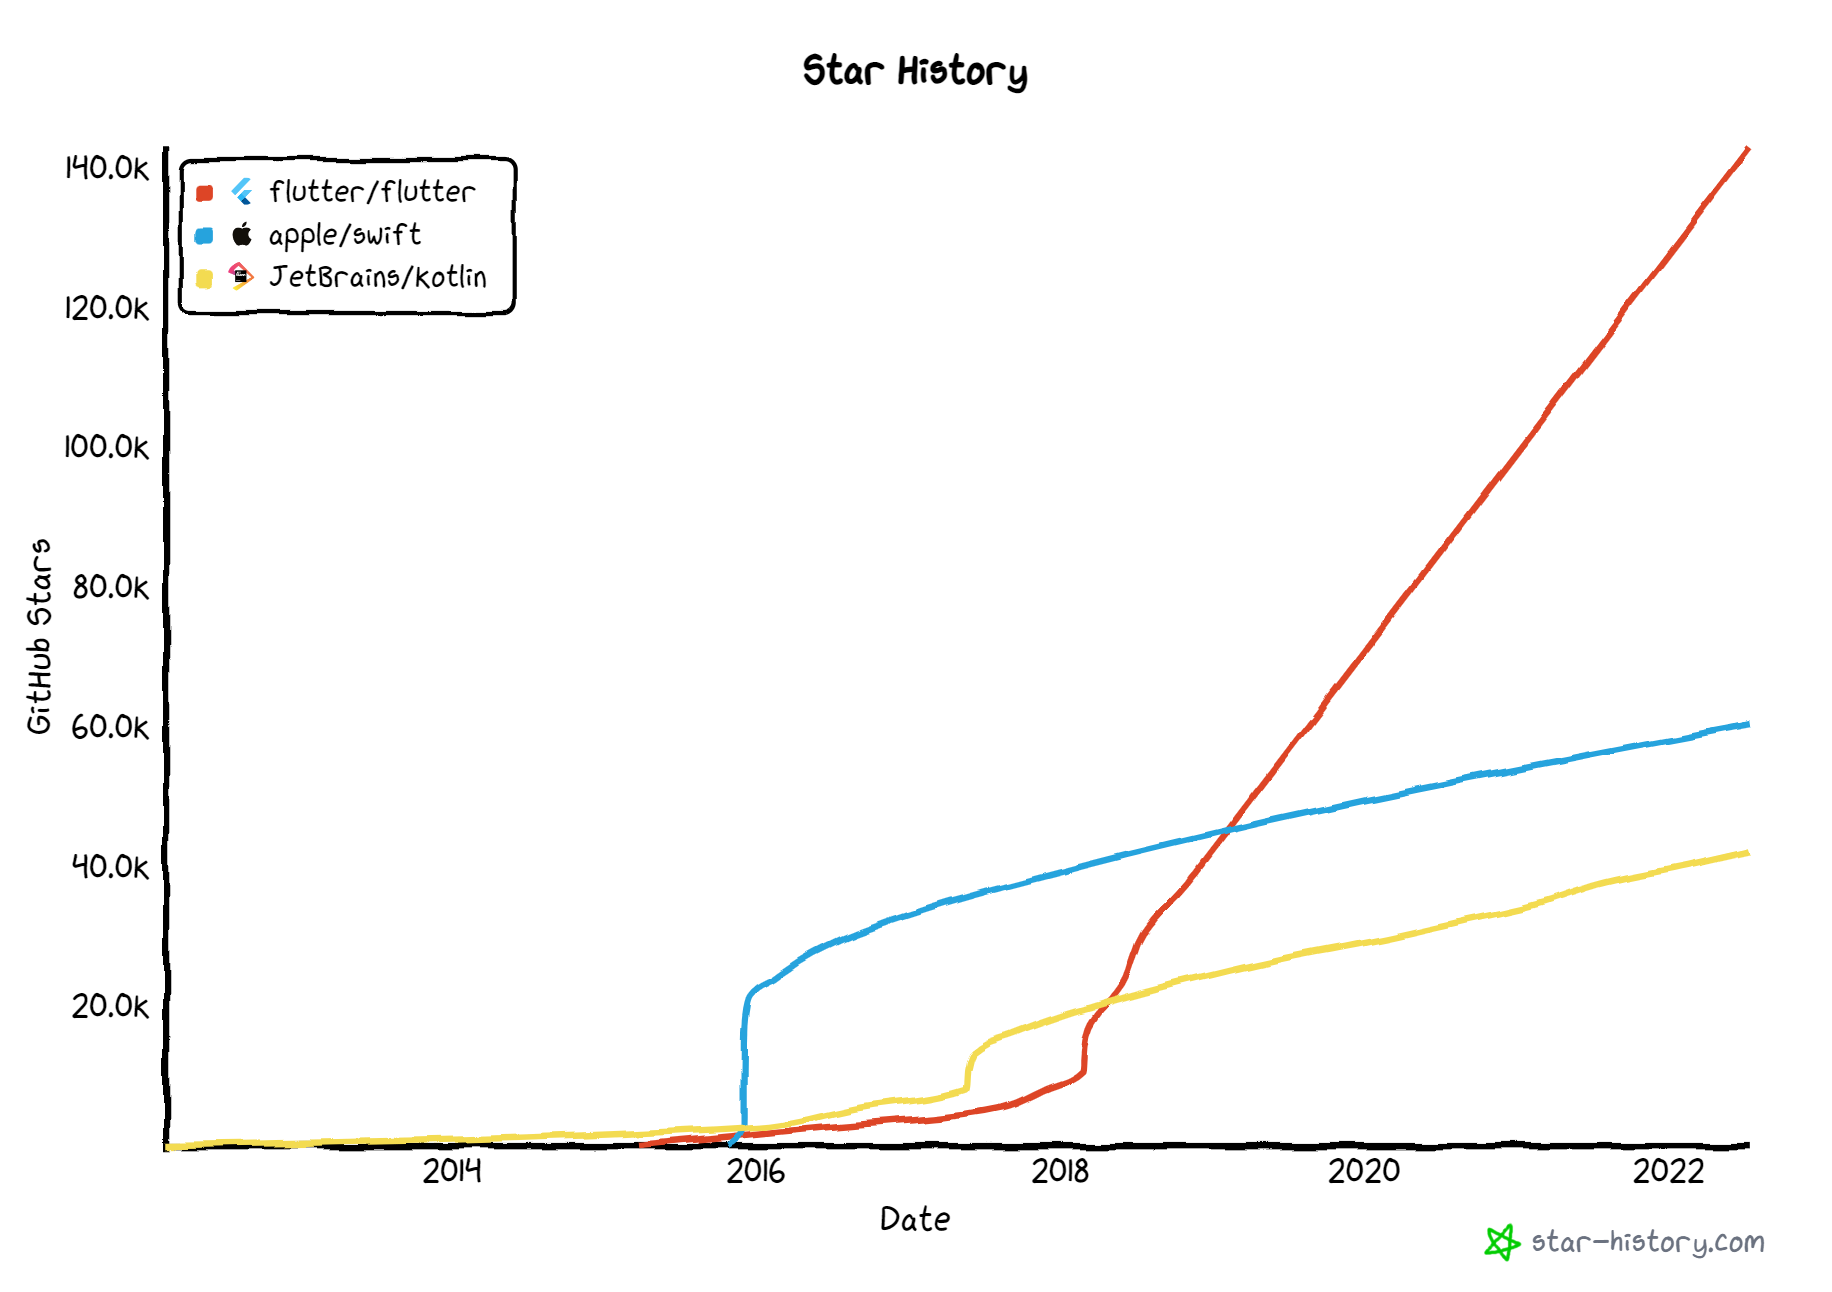
\includegraphics[height=8.5cm,keepaspectratio]{images/star-history_programming languages.png} 
  \caption[Zeitlicher Verlauf von Stars der Github-Repositorys von Swift, Kotlin und Flutter]{Zeitlicher Verlauf von Stars der Github-Repositorys von Swift, Kotlin und Flutter\protect\footnotemark }
  \label{fig:star_history}
\end{figure}
\footnotetext{\url{https://star-history.com/\#flutter/flutter\&JetBrains/kotlin\&apple/swift\&Date}}



Abbildung \ref{fig:star_history} zeigt ein, mit Hilfe der GitHub-Api erstelltes, Diagramm. Darin wird die Anzahl der Stars der Swift, Kotlin und Flutter Repositories im zeitlichen Verlauf angezeigt. 
Besonders gut zu erkennen ist, wie stark das Interesse an Flutter ist. Nach der ersten Ankündigung 2018 und der darauf ersten veröffentlichten Version ist die Zahl der Stars innerhalb von 4 Jahren auf 140 000 angestiegen. Die Repositories für Swift und Kotlin haben im gleichen Zeitraum gerade einmal 20 000 Stars dazu erhalten. Zwar haben Swift und Flutter beide innerhalb des ersten Jahres nach ihrer Vorstellung etwa 30 000 Stars erhalten. Jedoch ist das Interesse an beiden nach einer anfänglichen Phase abgeflacht und verlaufen parallel zueinander.

\subsubsection{Stackoverflow}
Ein anderer Anhaltspunkt für die Größe einer Entwicklergemeinschaft ist die Anzahl der gestellten Fragen auf Stackoverflow. Stackoverflow bietet eine Plattform, um Fragen zu Entwicklungsproblemen zu stellen. Diese können von anderen Entwicklern beantwortet werden. So können generelle Ideen diskutiert und kleine Code-Stücke ausgetauscht werden. Stackoverflow ermöglicht es angemeldeten Nutzern, unter entsprechender Filterung, die Anzahl der gestellten Fragen für einen Suchbegriff zu bestimmen. Hierfür wurde die Anzahl der Fragen bezüglich Kotlin, Swift und Flutter innerhalb der letzten 2 Jahre bestimmt. Zusätzlich wurde auch noch die Anzahl der ingesamt gefundenen Fragen bestimmt. Dabei wurden eventuelle Überschneidungen mit anderen Programmiersprachen, sowie unbeantwortete Fragen heraus gefiltert.

\begin{table}[ht]
\centering
\caption{Anzahl gefundener Fragen pro Programmiersprache}
\begin{tabular}{ |p{3.7cm}||p{5cm}| p{5cm}|}
 \hline
 Programmiersprache & Anzahl gefundener Fragen der letzten 2 Jahre & insgesamt gefundene\\
 \hline
 Kotlin &  105 082 Fragen\tablefootnote{Filter: [kotlin] or [android][kotlin] or [android]-[flutter]-[java] lastactive:2y.. is:question answers:1..} & 920 585 Fragen\\
  \hline
 Swift  & 71 749 Fragen\tablefootnote{Filter: [swift] or [ios][swift] or [ios]-[flutter]-[objectivc] lastactive:2y.. is:question answers:1..} & 670 697 Fragen\\
  \hline
 Flutter & 77 568 Fragen\tablefootnote{Filter:[flutter] or [dart] -[ubuntu] lastactive:2y.. is:question answers:1..} & 115 533 Fragen\\
 \hline
\end{tabular}
\label{tab:evaluations_questions_stackoverflow}
\end{table}

Tabelle \ref{tab:evaluations_questions_stackoverflow} zeigt die ermittelten Werte. Flutter hat hierbei in den letzten zwei Jahren eine ähnlich aktive Community wie Kotlin und Apple. Hier muss jedoch bedacht werden, dass Fragen, die bereits vor dem Untersuchungszeitraum gestellt wurden, innerhalb dieses Zeitraumes nicht erneut gestellt wurden. Deswegen wurde die insgesamt Anzahl der Fragen ebenfalls betrachtet. Hierbei ist die Anzahl sowohl bei Kotlin als auch Swift deutlich höher. Jedoch wurde diese beiden Technologien früher als Flutter veröffentlicht.
Für Flutter zeigt sich, dass in den letzten 2 Jahren eine ähnlich große Community wie für Kotlin und Swift existiert.

\subsubsection{Dokumentation}
Ein weiterer Faktor ist die Dokumentation. Sowohl Flutter als auch Kotlin und Swift veröffentlichen eine umfangreiche und von den Entwicklern dauerhaft aktualisierte Dokumentationsseite. Jedoch besitzt Flutter im Gegensatz zu Android und iOS einen offiziellen zentralen Ort\footnote{\url{https://pub.dev/}}, um nach externen Packages zu suchen. Hier sind neben den offiziellen von Flutter veröffentlichten Repositories, auch von der Community entwickelte Packages verlinkt. In der Summe können hier bereits über 27000 Erweiterungen gefunden werden\footnote{\url{https://pub.dev/packages?q=}}. Neben einem Punktesystem, dass diese bezüglich der Einhaltung von Richtlinien bewertet, werden außerdem die unterstützten Plattformen angezeigt. Zwar gibt es auch Bemühungen ein solches Verzeichnis für Kotlin und Swift einzuführen, jedoch sind diese nicht offiziell von den Entwicklerfirma betrieben und oft nicht vollständig.

Neben der Dokumentation für die Programmiersprache, existieren weitere Dokumentationen für die verschiedenen Entwicklungsansätze. Dabei sind sowohl für den cross-kompilierte, als auch für den native Ansatz eine umfangreiche Dokumentation verfügbar, da sie der Standardentwicklungsmethode der Programmiersprache folgen. Für den gewählten hybriden Ansatz konnte anhand von Anleitungen und Dokumentation der Programmiersprache eine ausreichende Basis gefunden werden. Lediglich der gemischte Ansatz verfügte über keine Dokumentation. Zwar existiert gute Dokumentation für die gewählten Grundlagen und die Web Implementierung, jedoch ist nur wenig Dokumentation für den genauen Ansatz und die Kombination der Technologien vorhanden. Dies wird jedoch durch die Art der Implementierung bedingt, da viele verschiedene gemischte Implementierungen möglich sind. Diese besitzen dabei oft eher einen experimentellen Charakter.

Zusammenfassend wird ersichtlich, dass bei einer normalen Nutzung der Programmiersprache beziehungsweise des Frameworks, eine umfangreiche Dokumentation gefunden werden kann. Je mehr sich jedoch von der normalen Nutzung entfernt wird, desto geringer wird die Dichte an verfügbaren Materialien. 

\subsubsection{Entwickler}
Ein letzter Faktor der zu dieser Kategorie analysiert werden soll, ist die Anzahl der verfügbaren Entwickler. Eine Befragung \cite{statist_used_programming_languages} von 71 547 Entwicklern der Firma Stackoverflow zeigt, dass etwa 9\% Kotlin, 7\% Dart und 5\% Swift beherrschen.
Bei den Programmiersprachen der Webtechnologien, gaben  65\% an, JavaScript zu kennen und 55\% können mit HTML beziehungsweise CSS entwickeln. Diese Zahlen lassen den Schluss zu, dass die Ansätze mit einem hohen Anteil an Web Technologie einen Vorteil haben, da es mehr Entwickler für diese Ansätze gibt. Jedoch wird auch bei diesen Ansätzen mindestens ein Entwickler benötigt, der sich mit den einzelnen Plattformen genauer auskennt. 
Ansonsten ist die Entwicklung eigener plattformspezifischer Funktionalität nicht möglich.

\section{Entwicklungsdauer}
Ein weiteres wichtiges Kriterium bei der Wahl des Ansatzes ist die Entwicklungsdauer, da diese sich auf die Kosten der entwickelten Multi-Plattform-Anwendung auswirkt. Außerdem sollen Applikationen möglichst schnell entwickelt und an den Nutzer verteilt werden können. Daher soll zusätzlich die Zeit betrachtet werden, bis die Applikation beziehungsweise ein Update bei den Nutzern verfügbar ist.

\subsubsection{Programmieraufwand}
Die genaue Entwicklungsdauer ist stark von der Erfahrung der Entwickler und eventuell auftretenden Problemen während der Implementierung abhängig. Folglich ist ein Zeitvergleich hier nicht sinnvoll. Stattdessen soll die Anzahl der geschriebenen Programmzeilen / Lines of Code (LOC) betrachtet werden.
Dafür wurden die einzelnen Daten mit Hilfe des Statistics\footnote{\url{https://plugins.jetbrains.com/plugin/4509-statistic}} Plug-In von JetBrains gesammelt.
Bei den beiden Implementierungen mit Web-Anteil wurde außerdem der notwendig Teil der Web-Implementierung mit angegeben. 
Die gesammelten Daten wurden in drei Teile aufgeteilt: Konfiguration, Benutzeroberfläche und Logik. 
Bei den Implementierungen, welche Flutter benutzen, ist der UI- und Logikcode zusammengefasst, da dies bei Flutter nicht unterschieden werden kann.
Als weiterer Parameter wurde der benötigte Code untersucht, um eine Liste an Objekten anzuzeigen.
Dabei wurde automatisch generierter Code nicht gezählt, sondern nur der tatsächlich geschriebene.

\begin{table}[ht]
\centering
\caption[Programmlänge der verschiedenen Implementierungen in LOC]{Programmlänge der verschiedenen Implementierungen in LOC}
\begin{tabular}{ |p{3.5cm}||p{2.5cm}|p{3.5cm}|p{2.5cm}|p{2.5cm}| }
 \hline
 Programmteile in Lines of Code & gemischte Applikation & cross-kompilierte Applikation & native\break Applikation & hybride\break Applikation \\
 \hline
 Gesamte\break Anwendung       &   2391(App) + 1533(Web) &   2100 & 3138 & 215(App) + 2814(Web)\\
  \hline
 Konfigurationscode  & 42 + 268& 32& 229& 30 + 357\\
  \hline
 Oberflächencode &\multirow{2}{*}{2349 + 1265}  &\multirow{2}{*}{2068}  & 1958& 86 + 1768\\
  \cline{1-1}
  \cline{4 -5}
 Funktionalität \& Logik & & & 951& 99 + 689\\
  \hline
 Beispiel: Liste an Gegenständen & 65(App) & 65 & 178 & 71(Web)\\
  \hline
\end{tabular}
\label{tab:lines_of_code}
\end{table}

Die in Tabelle \ref{tab:lines_of_code} zu sehende Aufschlüsselung zeigt, dass Flutter insgesamt die wenigsten Zeilen Code benötigt. 
Dabei werden gerade einmal 32 Zeilen Code Konfiguration benötigt. 
Der Rest sind knapp 2000 Zeilen Code mit Benutzeroberfläche und Logik.
Den höchsten Programmieraufwand in diesem Vergleich benötigt der gemischte Ansatz. Er kommt insgesamt auf circa 4000 Zeilen Code und benötigt damit rund doppelt so viel wie die Flutter Implementierung. 
Die native und die hybride Implementierung haben in etwa gleich viele Zeilen Code und liegen mit rund 3000 Zeilen Code zwischen den zwei anderen Implementierungen.

Bei dem zusätzlich betrachteten Beispiel, einer dynamischen Liste für Gegenstände ohne feste Länge, ist die Flutter Implementierung ebenfalls die Kürzeste. Dabei werden gerade einmal 65 Zeilen Code benötigt, wovon 55 Zeilen auf die Anzeige eines Gegenstandes und gerade einmal 10 Zeilen Code auf die Liste entfallen. Ähnlich verhält sich dies bei der Implementierung mit einer Webseite. Einzig die native Kotlin Applikation hat hierbei einen erhöhten Aufwand. Dabei fallen 75 Zeilen für das Design und weitere 83 Zeilen für die Steuerung der Liste an. Ein Großteil davon ist der Adapter, der benötigt wird, um die Liste zu steuern. 

Ebenfalls muss beachtet werden, wie viele Implementierungen je Ansatz benötigt werden. So ist bei dem gemischten und dem cross-kompilierten Ansatz lediglich die eine vorgestellte Implementierung nötig. Bei dem nativen Ansatz muss jedoch pro unterstützter Plattform eine eigenständige Implementierung erstellt werden. Bei der hybriden Applikation, wie sie in dieser Arbeit umgesetzt wurde, ist zwar die umgebende Applikation ebenfalls für jede Plattform zu implementieren, jedoch hat die Implementierung einen deutlich geringeren Umfang, da der Teil der Web-Anwendung lediglich einmalig zu programmieren ist.  

Es wurde gezeigt, dass eine cross-kompilierte Lösung mit Flutter deutlich weniger Zeilen Code als die anderen Implementierungen benötigt.
Sollte jedoch bereits eine Web-Anwendung existieren, reduziert sich der Implementierungsaufwand der hybriden Aufwand auf knapp 200 Zeilen Code und die gemischte Implementierung halbiert sich in etwa. Dadurch können diese beiden Implementierungen dann ebenfalls eine gute Alternative zu den anderen Ansätzen darstellen. Muss diese jedoch erst erstellt werden, ist gerade der gemischte Ansatz mit einem erhöhten Aufwand verbunden. Außerdem wurde festgestellt, dass mit mehr unterstützten Plattformen der native Ansatz sich im Aufwand multipliziert.

\subsubsection{Zeit bis zur Veröffentlichung der App und von Updates }
Die Entwicklungsdauer wirkt sich auch auf die Dauer bis zur Veröffentlichung einer ersten Version aus.
Je früher eine Anwendung veröffentlicht werden kann, desto früher können Kunden die Applikation nutzen und bei einer kommerziellen Nutzung folglich auch Umsatz produzieren.

Hier haben die gemischte und die hybride Implementierung den Vorteil, dass bei einer bereits bestehenden Webseite, die Zeit bis zur Veröffentlichung einer ersten Version sehr gering ist, da bereits wenige Zeilen Code die Webseite in der App anzeigen. Zu einem späteren Zeitpunkt können mehr Funktionalitäten und Optimierungen in kommende Versionen hinzugefügt werden. Wenn jedoch keine Webseite besteht, ist die anfängliche Dauer vergleichbar, beziehungsweise etwas höher als bei der cross-kompilierten Implementierung. Lediglich die native Implementierung benötigt durch das Erstellen der verschiedenen Plattform-Applikation deutlich mehr Zeit. Dies kann zwar durch zusätzliche Entwickler begrenzt werden, jedoch steigen dadurch die Entwicklungskosten.

Bei der Veröffentlichung von Updates zeigt sich ein weiterer Vorteil der Nutzung einer Webseite innerhalb einer Applikation. So können Updates auf der Webseite sofort verteilt werden und müssen nicht über den App-Store der verschiedenen Geräte verteilt werden. Die Veröffentlichung von Apps oder deren Updates kann dabei zwischen einem Tag und einer Woche dauern\footnote{\url{https://developer.apple.com/app-store/review/}} \footnote{\url{https://qr.ae/pvu0ud}}. Diese Zeit wird dafür bei jeder Änderung an der App bei allen vier Ansätzen benötigt.

\section{Benutzeroberfläche}
Die Bewertung einer Benutzeroberfläche ist stark von den persönlichen Präferenz abhängig. So empfinden Nutzer unterschiedlich, was eine gute Benutzeroberfläche ausmacht. Folglich soll in dieser Arbeit nicht auf das genaue Aussehen eingegangen werden, sondern auf einige allgemeine Eigenschaften der unterschiedlichen Benutzeroberflächen.

\subsubsection{Aussehen der Applikationen}
Grundsätzlich ist das Aussehen der Applikation vor allem davon abhängig, wie viel Zeit investiert wird, um ein angestrebtes Design zu erhalten. Um die unterschiedlichen Startseiten vergleichbar zu halten, wurde deswegen eine Maximalzeit für die Verwirklichung des Design festgelegt. Diese Maximalzeit orientiert sich an der benötigten Entwicklungszeit der entsprechenden Web-Ansicht. Dafür wurde außer für den Schriftzug mit Farbverlauf keine externen Design-Pakete oder Erweiterungen benutzt. Eine zusätzliche Anforderung war dabei, dass die Seiten für unterschiedliche Bildschirmgrößen benutzbar sein müssen.

\begin{figure}[ht]
  \centering
  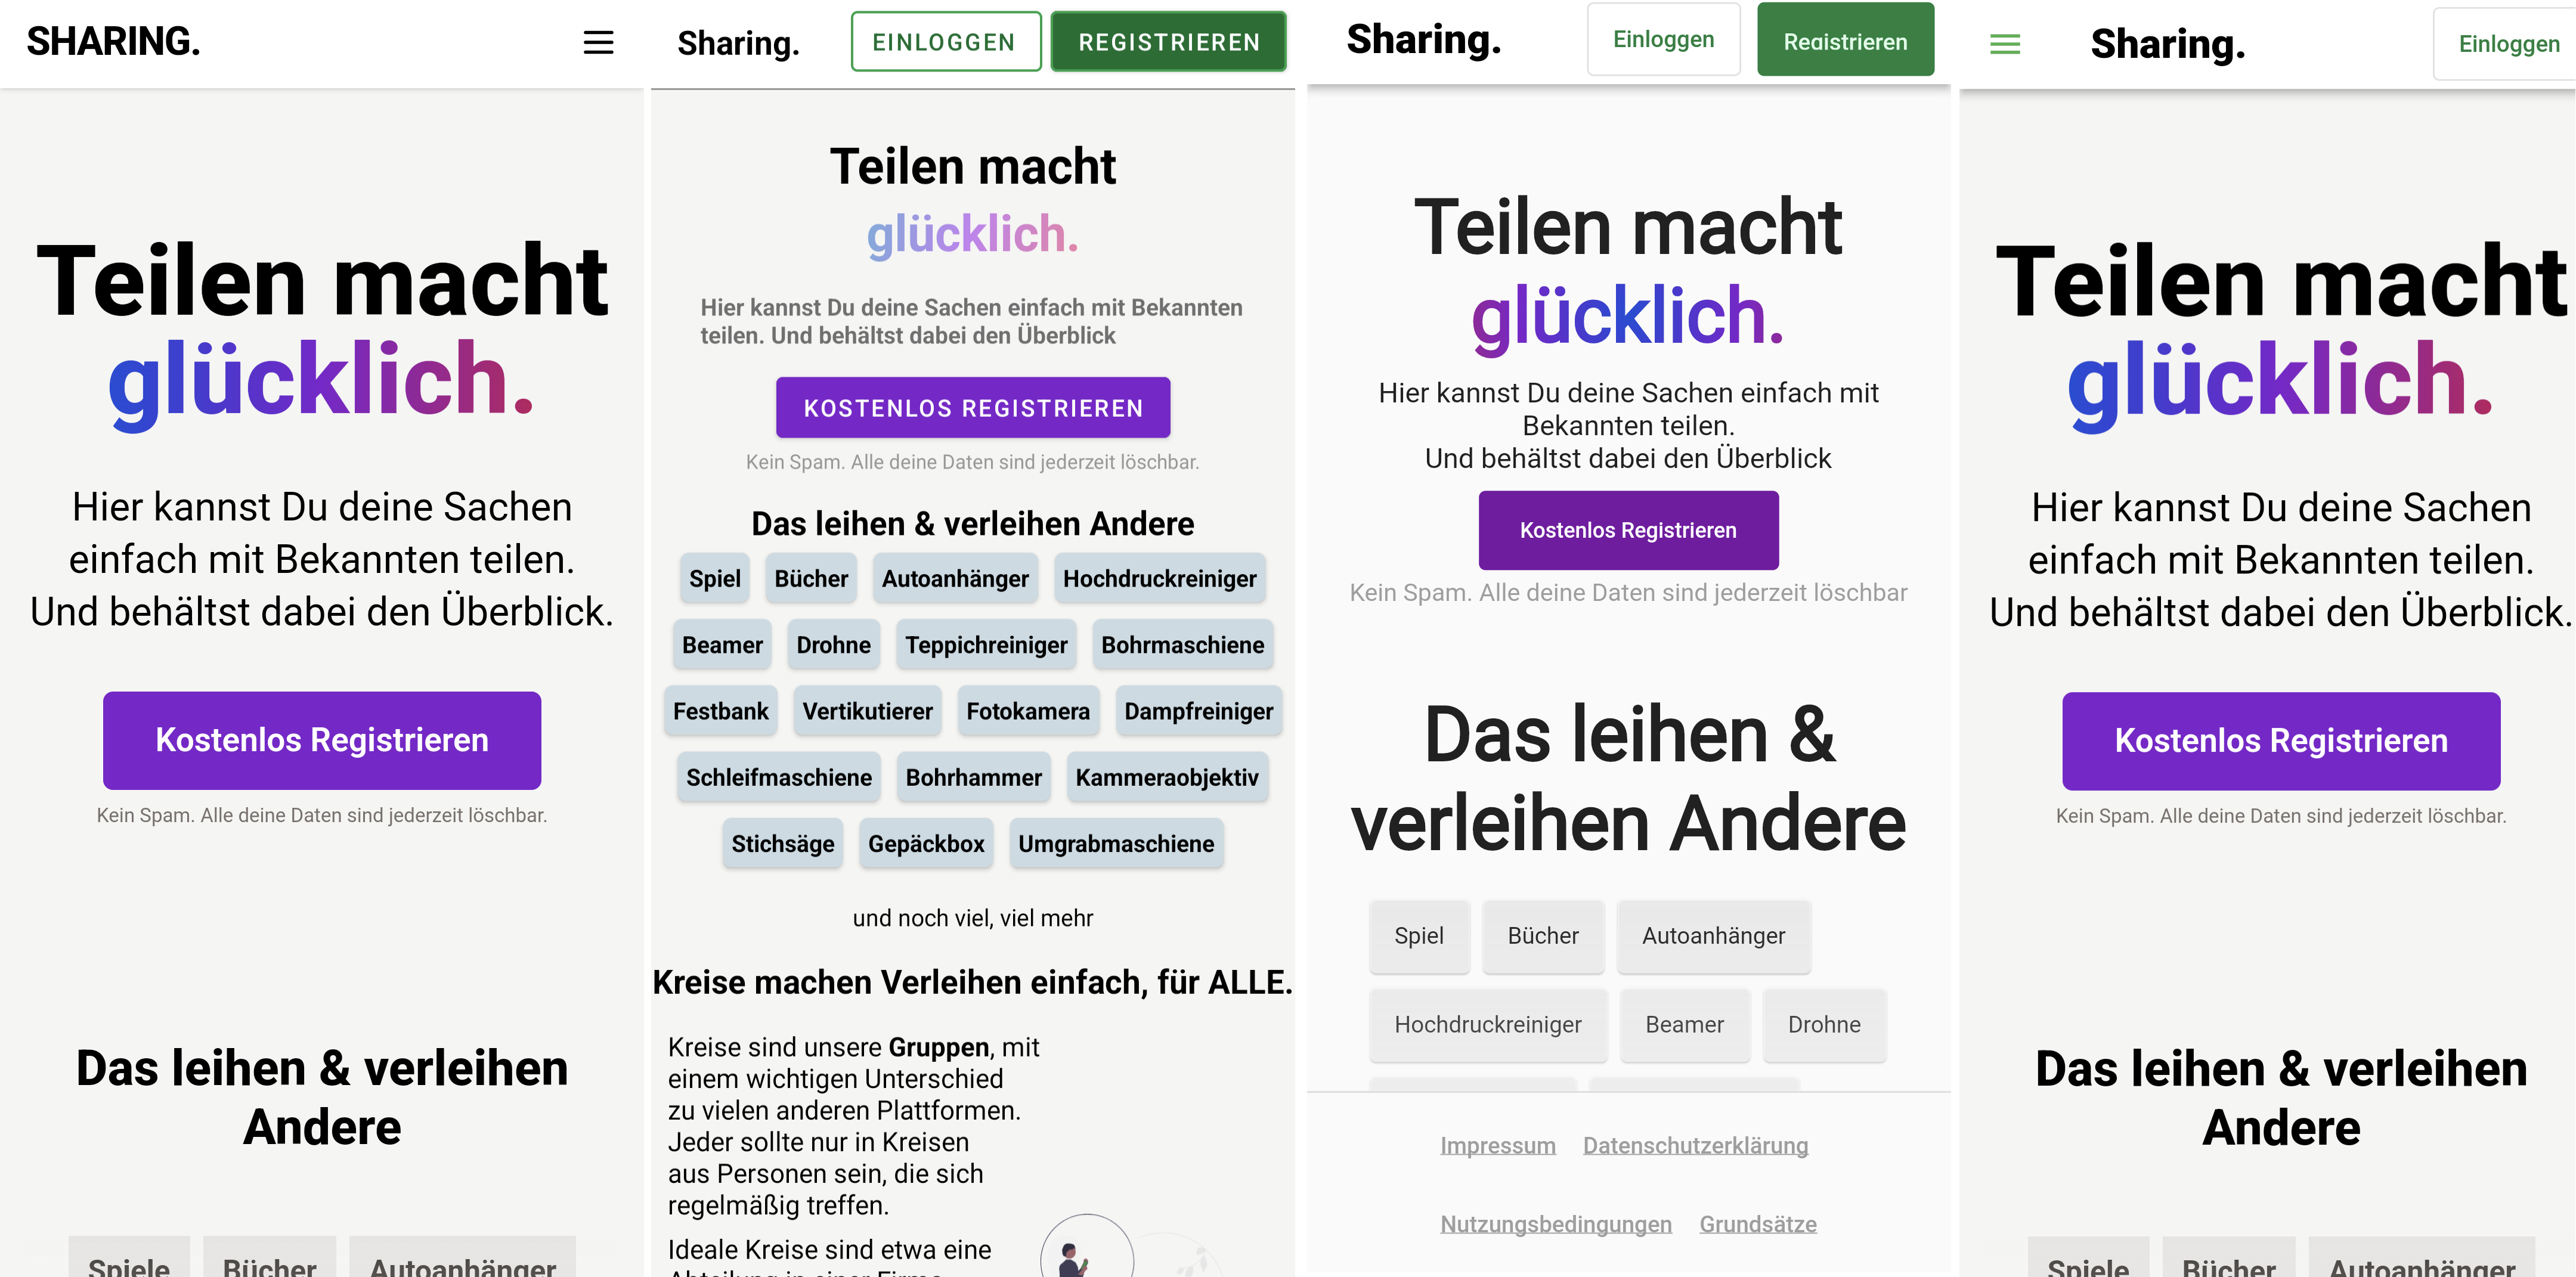
\includegraphics[height=7cm,keepaspectratio]{images/Startbildschirm_vergleich.png} 
  \caption[Vergleich des Startbildschirms der Implementierungen]{Vergleich des Startbildschirms der Implementierungen.\break Von links nach rechts: Hybride-Applikation, native Kotlin Applikation, Flutter Cross-Plattform-Applikation, Flutter Hybride Applikation}
  \label{fig:startscreen}
\end{figure}

In Abbildung \ref{fig:startscreen} sind die Startbildschirme der verschiedenen Anwendungen zu sehen. Dabei zeigen das erste und letzte Bild die Startseite der Webseite. Die zwei mittleren Bilder zeigen die im App-Code definierten Seiten. Grundsätzlich kann dabei festgestellt werden, dass die Seiten ähnlich aussehen, lediglich die Größe des Textes unterscheidet sich zwischen den Versionen stark.

Bei dem ersten Bildschirm, welcher von der hybriden Applikation stammt, musste am Design der Applikation nicht viel angepasst werden, da die Webseite bereits für die Nutzung an ein mobiles Endgerät angepasst war. Jedoch fallen bei der Benutzung Unterschiede zur nativen beziehungsweise Flutter Entwicklung auf. 
Um dies zu verdeutlichen zeigt Abbildung \ref{fig:sidemenu} die Seitenmenüanzeigen der Flutter-Anwendung (links) und der Webimplementierung (rechts). Hierbei ist klar zu erkennen, dass die Web-Implementierung für PC Nutzer ausgelegt ist, da das Menü für eine Anklick-Bedienung optimiert ist. 
Im Gegensatz dazu kann das Seitenmenü bei der Flutter Implementierung über eine Wischgeste geöffnet werden und wird dabei über den gesamten Gerätebildschirm angezeigt, während bei der Webseite das Menü nur innerhalb des Web-Containers angezeigt wird. Dadurch erhält der Nutzer in der Flutter Applikation den Eindruck, dass sich das Menü über die restliche UI legt. 
\begin{figure}[ht]
  \centering
  \includegraphics[height=7cm,keepaspectratio]{images/Seitenmenü_vergleich.png} 
  \caption[Vergleich des Seitenmenüs der nativen und hybriden Applikation]{Vergleich des Seitenmenüs bei nativer Implementierung (links) und JavaScript Implementierung (rechts)}
  \label{fig:sidemenu}
\end{figure}

Während auf der Webseite eine umfangreiche Design-Implementierung genutzt wurde, um das Aussehen der Anwendung zu verändern, wurden bei der nativen Kotlin und den Flutter Implementierungen lediglich die Farben und Textgröße angepasst. Dies wurde gemacht, um einen Eindruck für die Standardkonfiguration des Design der verschiedenen Implementierungen vergleichen zu können. Bei der Flutter Implementierung wirken die Elemente im Gegensatz zur nativen Implementierung moderner und besser an ein Smartphone angepasst. Dies wird deutlich, wenn die Login-Seite verglichen wird.

\begin{figure}[ht]
  \centering
  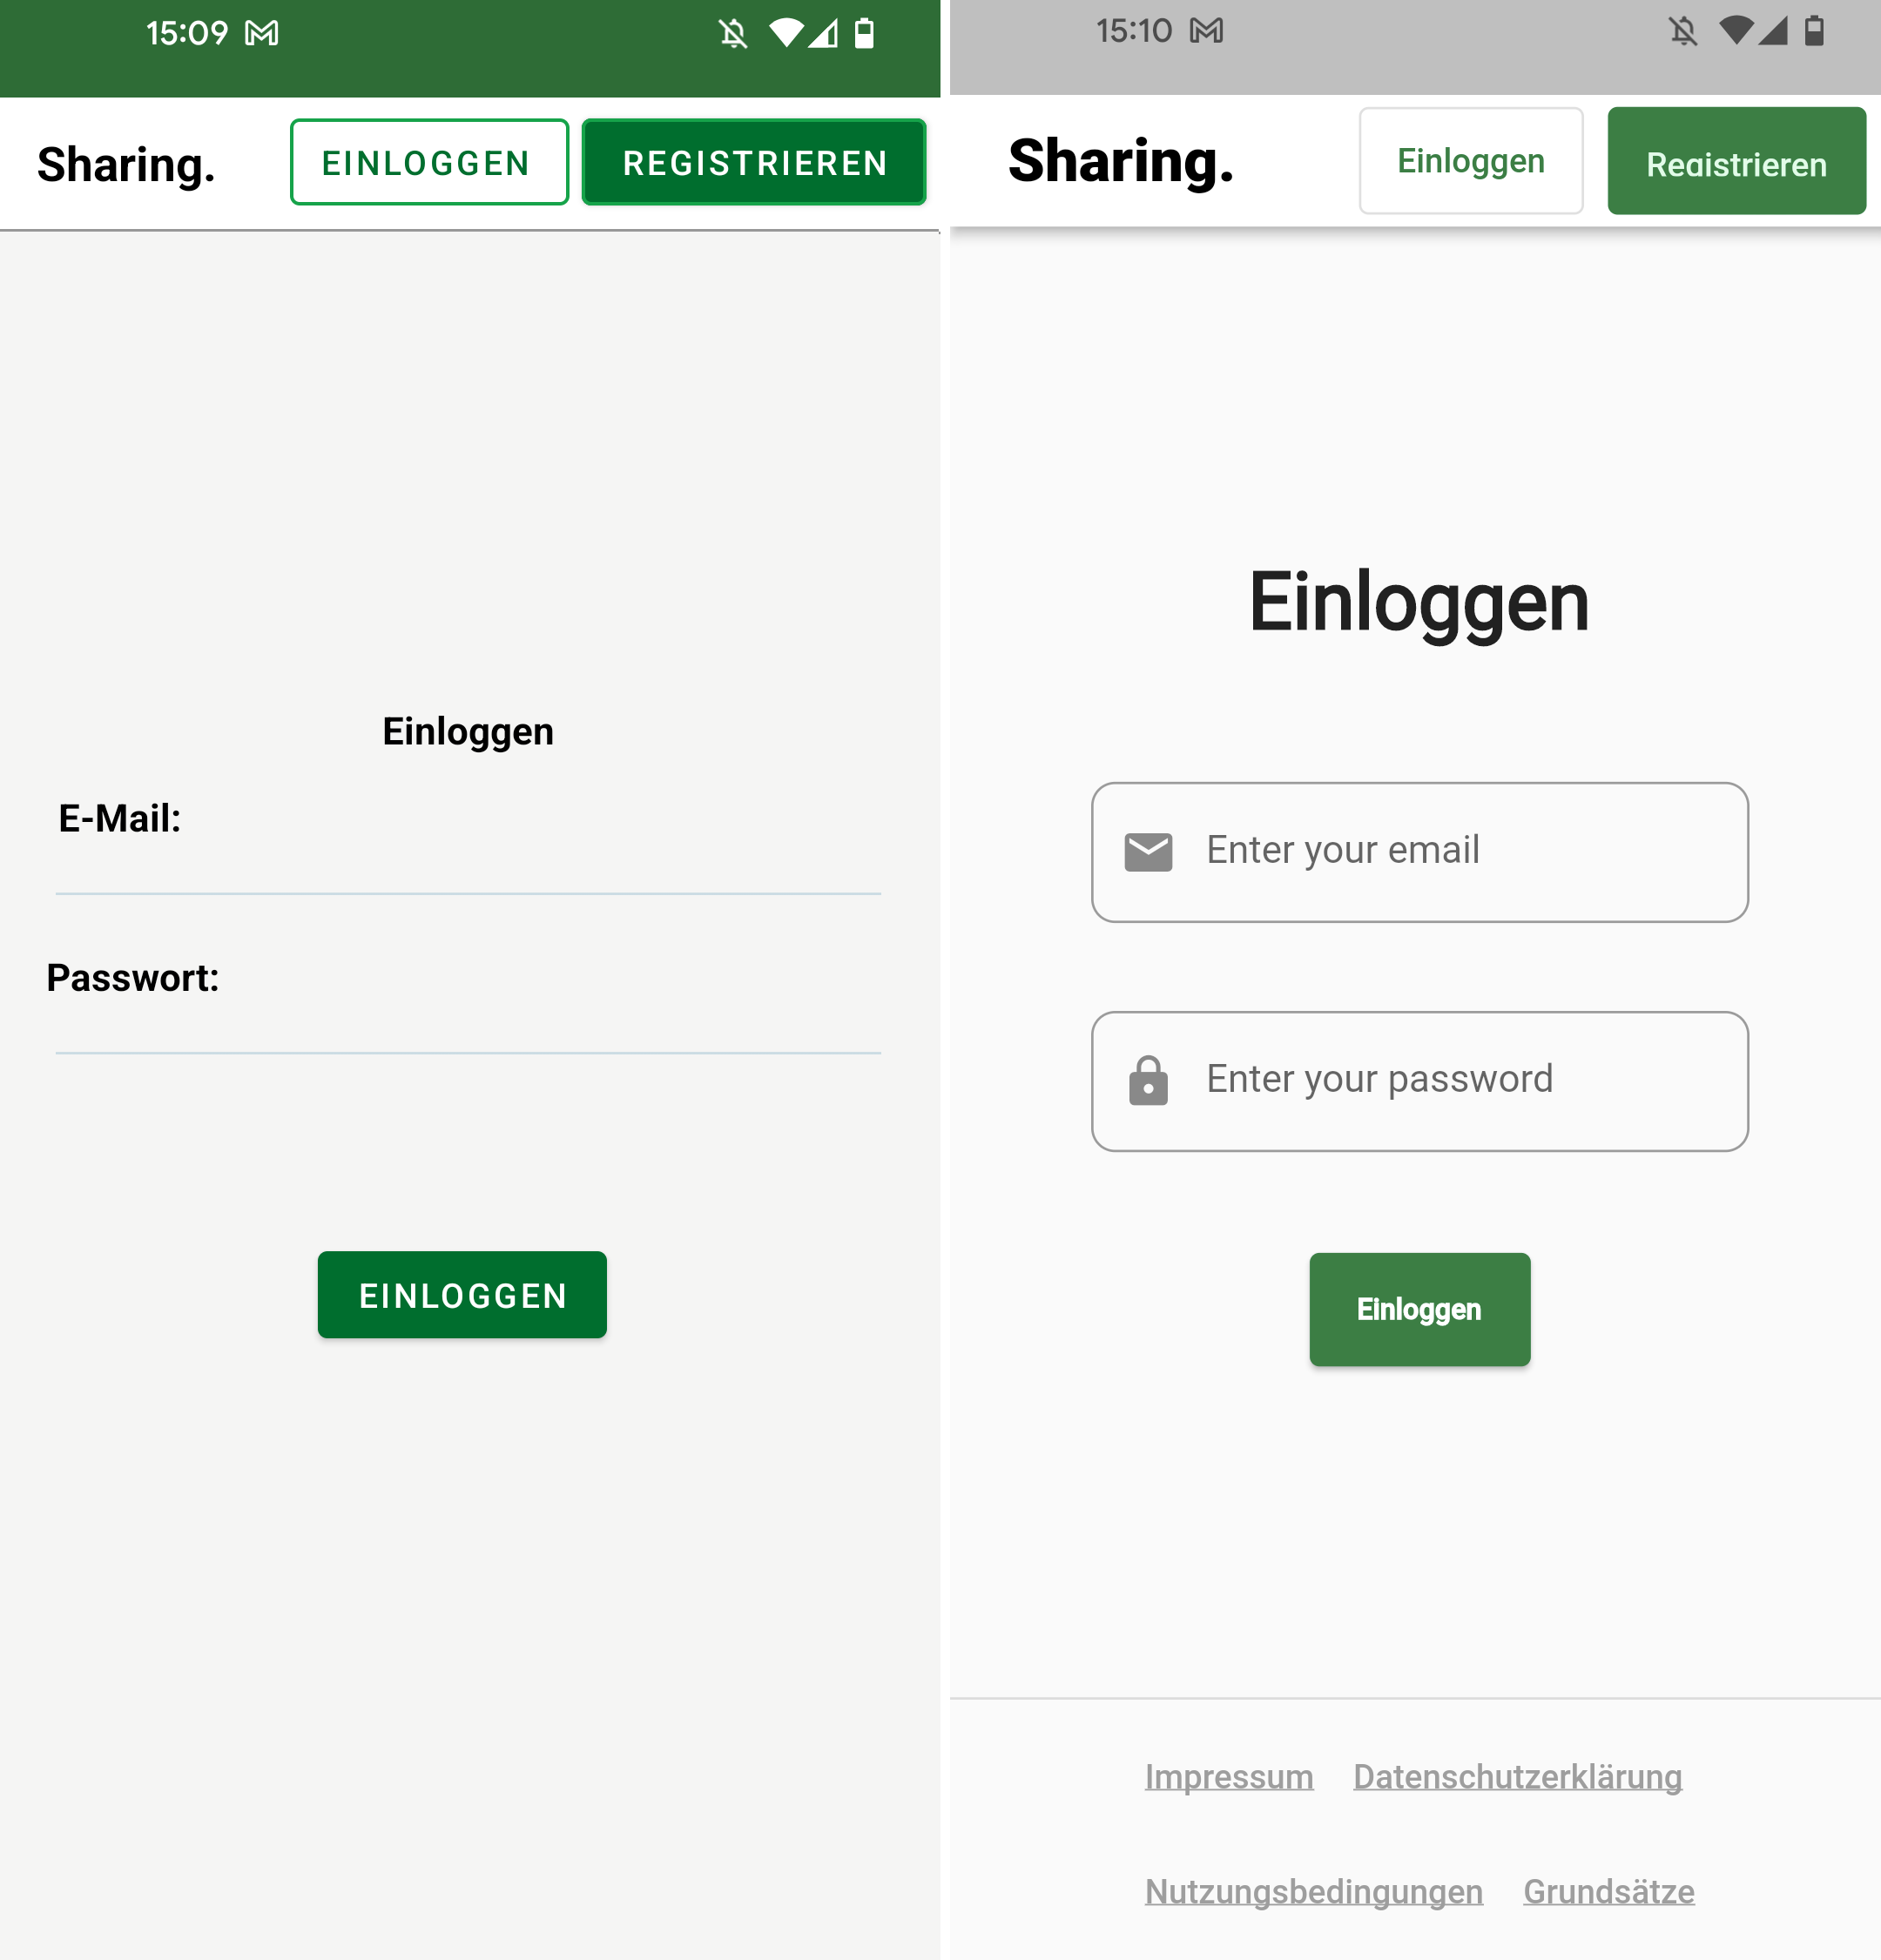
\includegraphics[height=7cm,keepaspectratio]{images/Login_vergleich.png} 
  \caption[Vergleich des Login-Bildschirms von Kotlin und Flutter Implementierung.]{Vergleich des Login-Bildschirms von Kotlin (links) und Flutter (rechts) Implementierung}
  \label{fig:loginscreen}
\end{figure}

In Abbildung \ref{fig:loginscreen} sind die Login-Seiten der nativen und des cross-kompilierten Ansatzes zu sehen. Dabei zeichnet sich Flutter durch ein besseres \"Out-of-the-Box\" Design-Paket aus. So ist das Input Feld bei der Koltin Implementierung  lediglich durch ein Strich definiert und kann dadurch für einen Nutzer schwer zu finden sein. Flutter hingegen hat als Standardinputfeld ein umrahmtes Feld, dass durch hinzufügen von Werten auf vordefinierten Attributen beliebig und einfach im Style angepasst werden kann. Bei der nativen Implementierung ist dies zwar ebenfalls möglich, allerdings entsteht dadurch zusätzlicher Aufwand.

Während der Entwicklung konnte festgestellt werden, dass mit genügend Zeit und den richtigen Erweiterungen, jede Benutzeroberfläche in das gewünschte Format zu bringen ist. Vor allem bei der Unterstützung unterschiedlicher Bildschirmgrößen benötigte jedoch die native Anwendungen umfangreiche Anpassungen, während dies bei den anderen Ansätzen deutlich unkomplizierter zu erreichen war. Flutter unterstütze die Verwirklichung einer gut aussehenden Benutzeroberfläche insofern, dass die Standardkonfiguration Googles Design-Paket Material3\footnote{\url{https://m3.material.io/}} nutzt.

\subsubsection{Konsistenz über Plattformen hinweg}
Ein weiteres Ziel bei der Entwicklung der Benutzeroberfläche ist die Konsistenz über Plattformen hinweg.
Dabei soll der Nutzer keinen Unterschied bemerken, wenn er von einer Plattform zur anderen wechselt. 
Das Risiko solcher Inkonsistenzen ist bei unterschiedlichen Implementierungen für die einzelnen Plattformen höher, als wenn eine einzelne Code-Basis verwendet werden kann.

Dementsprechend haben Implementierungen, die für mehrere Plattformen wieder verwendet werden können einen positiven Einfluss auf die Konsistenz.
Auf die in dieser Arbeit vorgestellten Implementierungen bezogen, bedeutet dies, dass die reine native Implementierung eine höhere Gefahr von Inkonsistenz besitzt, als die Hybride, Gemischte oder Cross-kompilierte.
Dabei ist zu erwähnen, dass auch die nativen Applikationen einen hohen Grad an Konsistenz erreichen können. Dies erfordert jedoch wieder einen höheren Aufwand und eine enge Zusammenarbeit der Entwickler während der Implementierung der verschiedenen Plattformen.

\section{Funktionalität}
Als letztes Kriterium wird die Funktionalität der einzelnen Ansätze betrachtet. Dabei soll neben der Plattformabdeckung, die Möglichkeiten zur Nutzung von offline Funktionalität und Plattformfunktionalität betrachtet werden.

\subsubsection{Plattformabdeckung}
Wie bereits erwähnt, sind nativ entwickelte Applikationen immer nur für eine Plattform verwenbar. Sie haben dementsprechend auch wenig wiederverwendbaren Code. Allerdings kann für jede Plattform eine native Applikation geschrieben werden und folglich können alle Plattformen abgedeckt werden.

Bei der hybriden Implementierung muss ebenfalls eine Applikation für jede Plattform geschrieben werden, jedoch kann der Web-Code auf den unterschiedlichen Plattformen wiederverwendet werden. Grundsätzlich können auch bei diesem Ansatz alle Plattformen unterstützt werden, dabei müssen jedoch die Anforderungen der verschiedenen App-Stores beachtet werden. Denn wie bereits erwähnt, verlangt beispielsweise Apple, dass Apps den Großteil der Funktionalität intern abbilden. Eine Implementierung, wie sie hier vorgestellt wurde, würde wahrscheinlich abgelehnt werden.

Flutter bietet eine Unterstützung für alle aktuell verfügbaren mobilen Plattformen an. Außerdem arbeiten sie an einer Möglichkeit, Flutter auch auf Embedded-Geräten auszuführen\footnote{\url{https://flutter.dev/multi-platform/embedded}}.
Somit können alle Plattformen abgedeckt werden. Jedoch kann die Plattformunterstützung der eigenen Applikation durch genutzte Bibliotheken eingeschränkt werden. Beispielsweise war die, in dieser Arbeit vorgestellte, cross-kompilierte Implementierung lediglich mit fünf der sechs Plattformen kompatibel, da der genutzte GraphQL-Client keine Web-Version unterstützt.

Die gemischten Implementierung unterstütze noch weniger Plattformen. So konnte aufgrund des genutzten Web-Containers die Applikation lediglich auf Android und iOS genutzt werden.
Daher ist es eventuell sinnvoll, vor der Wahl eines Ansatzes auch benötigte Technologien zu recherchieren und die verfügbaren Bibliotheken zu analysieren, um derartige Probleme bereits vor dem Start der Implementierung zu identifizieren.


\subsubsection{Offline Funktionalität}
Es gibt einige Fälle in denen der Nutzer eine Applikation benutzen will, auch wenn er aktuell über keine aktive Internetverbindung verfügt. In diesem Fall benötigt die Applikation eine offline Funktionalität.

Wie in dieser Arbeit erwähnt, sind die Implementierungen die eine Webseite als Teil ihrer Implementierung haben offline stark eingeschränkt oder haben keine Funktionalität. Im Falle der gemischten Implementierung kann eine offline Funktionalität zumindest teilweise erreicht werden, indem bei einer fehlenden Internetverbindung durch Flutter implementierte Seiten angezeigt werden. Die native und cross-kompilierte Lösung haben hier den Vorteil, dass ihre Benutzeroberfläche unabhängig von einer aktiven Internetverbindung nutzbar ist. Zwar kommen die angezeigten Daten von einem Server, jedoch können diese lokal zwischengespeichert werden. Diese Lösung ist dabei sowohl für die native, kross-compilierte und gemischte Implementierung möglich. 

Zu beachten ist, dass einige hybride Frameworks Daten und Benutzeroberfläche lokal auf dem Gerät speichern und dadurch eine offline Funktionalität möglich wäre. Allerdings verschwinden dadurch die Vorteile der Nutzung einer online Version, wie etwa die einfache Verteilung von Updates.

\subsubsection{Nutzung von Plattformfunktionalität}
Wie bei der Vorstellung der unterschiedlichen Implementierungen aufgezeigt wurde, kann mit der richtigen Implementierung die Nutzung der Plattformfunktionalität bei jeder der vier Implementierungen ermöglicht werden. Jedoch konnte aufgezeigt werden, dass die Nutzung mit unterschiedlichen Aufwand verbunden ist. So ist dies bei der nativen Implementierung am einfachsten umsetzbar. Auch der cross-kompilierte und der gemischte Ansatz können vollständig, wie in Kapitel 4.3.3 vorgestellt, auf die nativen Funktionen zugreifen. Ebenfalls kann der hybride Ansatz native Funktionalität nutzen, muss dafür jedoch eine Javascript-Schnittstelle nutzen. Dies birgt Gefahren, die beachtet und abgeschätzt werden müssen (siehe Kapitel 4.2.2). Hier hat der gemischte Ansatz insofern den Vorteil gegenüber dem hybriden, dass die Web-Ansichten, die Plattformfunktionalität benötigen, durch Flutter-Seiten ersetzt werden können. Somit ist ein sicherer und einfacher Zugriff wie bei der cross-kompilierten Implementierung möglich.

\chapter{Fazit}
\section{Flutter vs. Native Android}
\section{Nativ vs. Hybrid vs. Cross-Plattform}

\section{Entscheidung zu unterschiedlichen Ansätzen}

------
Schon genauere Erklärung:
Wenn man die Idee zu einer App hat, gibt es die große Frage, wie man nun anfängt und welche Programmiersprache / Framework man wählt. Hierfür gibt es ganz verschiedene Ansätze.  

Jedoch noch grundlegender ist die Frage nach der Plattform. Es gab lange Zeiten in der Applikationsentwicklung, dass nur eine Webversion veröffentlicht wurde. Mittlerweile nutzen jedoch viele Menschen nur noch ihr Smartphone und wollen dementsprechend auch nur mit mobilen Versionen auskommen. Man kann natürlich auch im Web veröffentlichte Applikationen auf dem Handy nutzen, jedoch gibt es hier zwei Sachen, die dazu führen können, dass man eine eigenständige App entwickelt.
1. Eine auf mobile angepasste UI. - Auch wenn es heutzutage in fast jedem Framework und vor allem in den gängigen UI-Frameworks verschiedene Ansätze gibt, die eine recht nutzerfreundliche Version für Mobilgeräte anbieten, oder manchmal auch sogar komplett eigenständige Oberflächen für mobil angezeigt werden, so kann es doch sinnvoll sein, nochmal extra angepasste UI in Form einer Applikation nativ für die Geräte zu entwickeln. Dadurch kann man gezielt Oberflächen für die Plattformen bauen und dabei auf Plattform eigene Design Unterstützungen zugreifen. Die eine Bedienung um einiges besser machen.
2. Nutzung von Hardwarefunktionalität. -  Ein noch viel wichtigerer Punkt ist es, Funktionalität die mobile Endgeräte anbieten, zu nutzen, die etwa auf einem PC nicht nutzbar sind. Dazu zählen unter anderem GPS-Nutzung, Kamerafunktionalitäten, Bluetooth-Verbindungen,.... Diese können zwar manchmal auch durch einen PC geboten sein, jedoch ist es hier nicht gegeben, während man bei einem Smartphone sicher davon ausgehen kann, dass die Kamera genutzt werden kann. So können einige Geschäftsprozesse der Applikationen vereinfacht oder umgestaltet werden, so dass eine Nutzung der Applikation für den Nutzer einfacher wird, bzw. es können auch neue Funktionalitäten daraus ergeben, die es eventuell davor nicht gab.

Wenn nun die Entscheidung getroffen wurde, dass man eine mobile Applikation entwickeln will, so gibt es nun verschiedene Ansätze bzw. Frameworks, die zur Verfügung stehen. Dabei gibt es viele verschiedene Frameworks die auf den ersten Blick das selbe tun, aber doch recht unterschiedlich sein können und unter gewissen Ummständen sich manche besser eignen als andere. 
Eine der ersten Fragen die dabei im Raum steht. Gibt es bereits eine Webversion der Applikation.
Wenn nicht, so kann es von Anfang an spannend sein, ein Framework zu wählen, dass wie Flutter eine Cross-Plattform-Applikation erzeugt, wo auch eine Webversion mit gehostet werden kann.
Falls es bereits eine Webversion geben, so geht der Weg eher in Richtung von Nativen- bzw. Hybriden Applikationen, da meißt nur noch einzelne Teile der Applikation entwickelt werden müssen. Dies ist jedoch auch kein Grund eine Cross-Plattform-Entwicklung auszuschließen, da dadurch nur ein Code geschrieben werden muss um etwa beide vorherschenden mobilen Plattformen abzudecken: iOS und Android.

'''Hier könnte man so ein Art Diagramm machen mit Fragen und dann Entscheidungswegen. So nach dem Motto finde dein Framework zur entwicklung einer mobilen Applikation.'''



\vfill
\pagebreak

\appendix

% ----------------------------------------------------------------------------------------------------------
% Abkürzungsverzeichnis (optional, bitte nur wenn sinnvoll)
% ----------------------------------------------------------------------------------------------------------
%\listoftables
\addchap{Abkürzungsverzeichnis}
\begin{acronym}[KDE]
\acro{BA}[BA]{Bachelorarbeit}
\end{acronym}
\vfill
\pagebreak


% ----------------------------------------------------------------------------------------------------------
% Filter fuer Literatur und Quellen definieren
% ----------------------------------------------------------------------------------------------------------

\defbibheading{Literatur}{\addchap{Literaturverzeichnis}} 
\defbibheading{Quellen}{\addchap{Internetquellenverzeichnis}} 
  
\defbibfilter{Literatur}{\not\keyword{online}} 
\defbibfilter{Quellen}{\keyword{online}} 


% ----------------------------------------------------------------------------------------------------------
% Literatur
% ----------------------------------------------------------------------------------------------------------

\printbibliography[heading=Literatur,filter=Literatur] 
\vfill

\pagebreak


% ---------------------------------------------------------------------------------------------------------- 
% Internetquellen 
% ---------------------------------------------------------------------------------------------------------- 

\printbibliography[title = {Quellenverzeichnis}, heading=Quellen,filter=Quellen] 

\pagebreak 

% ----------------------------------------------------------------------------------------------------------
% Anhang
% ----------------------------------------------------------------------------------------------------------
\appendix


\chapter{Anhang}

% \input{inhalt/suppl}


\pagebreak


% % ----------------------------------------------------------------------------------------------------------
% % Eigenschtändigkeitserklaerung
% % ----------------------------------------------------------------------------------------------------------
\thispagestyle{empty}
\chapter*{Erklärung zur Bachelorarbeit}

\bigskip
\bigskip 
\bigskip 

\textbf{1.}\\[1ex]
    Mir ist bekannt, dass dieses Exemplar der Abschlussarbeit als Prüfungsleistung in das Eigentum der Ostbayerischen Technischen Hochschule Regensburg übergeht.

\textbf{2.}\\[1ex]
    Ich erkläre hiermit, dass ich diese Abschlussarbeit selbständig verfasst, noch nicht anderweitig für Prüfungszwecke vorgelegt, keine anderen als die angegebenen Quellen und Hilfsmittel benutzt sowie wörtliche und sinngemäße Zitate als solche gekennzeichnet habe.

\bigskip 
\bigskip 
\bigskip 
~\hfill\begin{minipage}{.5\textwidth}

Regensburg, den \today

\bigskip 
\bigskip

\line(1,0){200}
\newline
\stud

\end{minipage}




\end{document}